\documentclass[12pt,a4paper,oneside,english]{UPBThesis}
\setcounter{secnumdepth}{3}
\setcounter{tocdepth}{3}
\usepackage{graphicx}
\usepackage[
  bookmarksnumbered,
  bookmarks,
  bookmarksopen=true,
  pdftitle={Dissertation},
  linktocpage,
  dvips]{hyperref}
\usepackage{amsmath}
\usepackage{amssymb}
\usepackage{inputenc}
\usepackage[T1]{fontenc}
\usepackage{algpseudocode}
\usepackage{algorithm}
\usepackage{tabularx}
\usepackage{array}
\usepackage{subfigure}
\usepackage{multirow}

\floatstyle{boxed}
\restylefloat{figure}
\algrenewcommand\algorithmicrequire{\textbf{input}}
\algrenewcommand\algorithmicensure{\textbf{output}}

\newcommand{\hctimes}[2]{{#1}\!\times\!{#2}}
\newcommand{\hcrange}[2]{\overline{{#1}\colon\!\!{#2}}}
\newcommand{\hcsignalspace}{\mathbb{R}^d}
\newcommand{\hcweightspace}{\mathbb{R}^w}
\newcommand{\hcdictspace}{\mathbb{R}^{\hctimes{w}{d}}}

\singlespacing

\begin{document}

\author{Horia COMAN}

\title{Text Detection and Deep Neural Networks}

\facultatea{Faculty of Electronics, Telecommunications and Information Technology}
\tiplucrare{Dissertation}
\domeniu{Applied Electronics and Information Engineering}
\catedra{Applied Electronics}
\campus{Leu}
\program{Advanced Curriculum Master Program in Imaging, Bioinformatics and Complex Systems (ITEMS)}
\titlulobtinut{Master of Science}
\director{Prof. Dr. Ing. Erhardt BARTH\\Prof. Dr. Rer. Nat. Thomas MARTINETZ\\As. Dr. Ing. \c{S}erban OPRI\c{S}ESCU}

\submissionmonth{September}
\submissionyear{2012}

\beforepreface
\listoffigures
\listoftables
\abbreviations {
  CNN = Convolutional Neural Network\\
  MP = Matching Pursuit\\
  OMP = Orthogonal Matching Pursuit\\
  OOMP = Optimized Orhtogonal Matching Pursuit\\
  PCA = Principal Component Analysis\\
  ZCA = Zero Component Analysis\\
  SVM = Support Vector Machine
}
%\preface{}
\afterpreface

\unnumberedsection{Stream of thought writing}

We focus more on coding methods. According to (cite Ng and guys here), this is the most important part in such a system. Dictionaries could well be random.

Some conventions: Vectors are written in boldface with lower case letters, like this $\textbf{v}$. Addressing elment $i$ is done with a subscript, like this: $\textbf{v}_i$. Accessing a set of element $\Lambda$ is done with a subscript, but using the whole set, like this: $\textbf{v}_\Lambda$. It is understood that the elements are produced in increasing index order. Matrices are written in boldface with capital letters, like this $\textbf{A}$. Accessing a certain column $i$ is done with a superscript, like this: $\textbf{A}^i$. Accessing a certain element $j$ in column $i$ is done with both a superscript and a subscript, like this: $\textbf{A}^i_j$. Accessing a certain subset of columns $\Lambda$ is done with a superscript, but using the whole set, like this: $\textbf{A}^\Lambda$. It is understood that the columns are produced in increasing index order. Accessing a certain subset of indices $\Lambda$ of column $i$ is done with both a superscript and a subscript, like this: $\textbf{A}^i_\Lambda$. It is understood that the elements are produced in increasing column order. Accessing a certain subset of indices $\Theta$ of a certain subset of columns $\Lambda$ is done using both a superscript and a subscript, like this: $\textbf{A}^\Lambda_\Theta$. It is understood that the columns are produced in increasing index order and the elements from each column are produced in increasing index order as well.am dar 

[[[Talk about typographic conventions]]]

This work presents several contributions: a general architecture for feature extraction for computer vision classification or regression, with a neural-network like structure, but much more general, a novel way of computing nonlinearities in it which produces state-of-the-art results on two benchmark image recognition tasks, a description of a text detection system, and experimental results with it and the two image recongnition tasks.

Text detection: we are given an input image, which contains several areas of text. The goal is to detect these areas and then perform OCR on them. The task however is harder than OCR as usually natural images are provided and text is written in a variety of fonts, on a variety of backgrounds, and filmed from a variety of positions, such that the classical OCR of top-down view does not hold. Ideally this should be solved in video and online.

The problem has been studied by other authors (cite them here) and in the context of deep learning (cite them here).

We assume throught the usage of the lating alphabet and left-to-right, top-to-bottom writing conventions.

This work shows how I built a system for text detection, using, as the title suggests, Deep Neural Networks.

First we'll consider the problem on a single image. The problem can be broken down into several steps: first, find the regions of the image where text is, then for each image, corresponding to a word, segment it into characters. Then, recognize each character. Finally, build a word from each image, considering the letters as well as spellcheck-type data which is a must.

The first subproblem is arguably the hardest. Suppose we have a general procedure which detects for a small image of size $\hctimes{p}{p}$ if that is a letter or a nonletter. Given such a procedure we run it over all patches found by centering each pixel. A new ``binary'' image is obtained which contains $1$ if the pixel $i,j$ is the center of a letter patch and $0$ otherwise. Several such images are built for varying values of $p$. This image gives a general indication of where the text is. Still, segmentation must be done, and, possibly oriented text segments must be generated from each image. In cases where a rectangle in one image overlaps with a rectangle in another, a method for specifying which has priority should be employed. This is a mostly hand-crafting engineering problem, and as such is solved in an heuristic way.

After segemntation, a series of images are produced from the original image, which contain the words. They still must be processed and understood.

The next step is thus the breaking of words into letters. The images we obtain will generally have a rectangular form, more wide than tall. We consider that a single row of letters is present, therefore segmentation only has to worry about the horizontal axis. If the image is of size $\hctimes{m}{n}$ then we have at most $n$ letters in it, in a very degenerate case, and at least one. This puts an upper bound on what we're about to do. We must also have a classifier here which knows how to separate into letters and the several punctuation marks common in words. This is a tougher classifier though and a probabilistic output would be nice for a Dynamic Programming approach to this.

Much of the actual work for this project has gone into building the classifier for letter/nonletter and then specific letters.

The classifier is based on a Convolutional Neural Network (CNN) (cite CNN here). However, it suffers some generalizations. Finally, we obtain a general coding system, neural network inspired, but not necesarily a classical network.

For the moment assume we are given the image $I$ of size $\hctimes{m}{n}$. This can be a patch from the original image we wish to classify as letter / nonletter or a segment of an extracted image for which we wish to find the actual letter. In any case, the task at hand is image recognition. It is a complex task. The naive approach of simply training a classifier on the raw image data will usually yield poor performance, except in the most simple of cases. Image classification systems therefore consist of two parts: a feature extraction phase and a proper classification phase. The goal of the first is to transform in an input image so as to be more easily handled by the latter phase. As the name suggest, it does so by ``extracting'' certain properties of an image, generically called ``features''. For example, a feature can be the amount of blue in the top of an image, or the variance in a small patch from the image, or the response to a oriented bandpass filter around a certain position etc. Extraction might mean a simple check for the presence or absence of the property, or might be a gradual percentace of presence of the feature in the image, or it might be computed in a whole other way. All the features amployed by a feature extraction layer form the ``feature set''. In general, the extraction process might not consider all features as independent, that is, a high presence of a feature in the set migth trigger a lower resulting presence of another feature. The input of the feature extraction phase is the image, $I$, and the output is a description of the feature set, usually called the ``feature vector'', and denoted by $F$, which contains one element for each feature in the feature set, and which thus codes the extraction result. For the latter stage, only $F$ is used.

Feature engineering, that is, the human-guided process of feature construction, is a big part of most machine learning applications. Usually, for best performance, deep knowledge of the problem domain must be coupled with an understanding of the Statistics and Machine Learning.

In the last decade, however, automatic feature construction, known as unsupervised feature learning (cite people here), has received much attention, producing systems with state of the art performance, and, in the field of Neural Networks, allowing the construction of so called Deep Neural Networks, which were thought impossible to build by standard methods (cite google and microsoft recent results with such networks). The whole field of Deep Learning deals with automatic feature extraction in one way or another.

\chapter{Overview of Feature Extraction}

In our framework, a feature is a small image patch - a filter - of some sort. The full feature set consists of $w$ normalized square images of size $d = \hctimes{p}{p}$ with $p < \min(m,n)$. We denote it by $\textbf{C} = \left[ \textbf{C}^1 \left|\right. \textbf{C}^2 \left|\right. \dots \left|\right. \textbf{C}^w \right] \in \mathbb{R}^{\hctimes{d}{w}}$. Normalization implies $\|\mathbf{C}^i\| = 1$ for all $i \in \hcrange{1}{w}$. For now we consider the feature set as given. Speaking broadly, though, feature sets can be generated randomly \cite{random-weights-feature-learning}, or taken to be a well-known set, such as DCT bases or Gabor Wavelet bases \cite{simple-method-sparse-coding}, or, even learned from a sample of patches extracted from the training set of the classification system \cite{emergence-sparse-coding,sparse-coding-strategy-V1,tiny-images}. More details about feature set construction will be given in the appropriate section.

A feature extractor is composed of a number of recoding modules, linked in a serial manner. The input image is propagated through these modules and transformed by them. The first such module starts with the image $\textbf{I}$ and produces a set of images $\{\textbf{I}_i^1\}_{i=1}^{l_1}$. The next module accepts as input $\{\textbf{I}_i^1\}_{i=1}^{l_1}$ and produces $\{\textbf{I}_i^2\}_{i=1}^{l_2}$. The last module outputs $\{\textbf{I}_i^k\}_{i=1}^{l_k}$, which is linearized to produce the feature vector $\mathbf{F}$. The stacking of these module produces a deep forward path for the input image. As we will see, this transformation can be modelled as a neural network. Hence the name Deep Neural Network. 

A module consists of several standard steps, called \emph{coding}, \emph{nonlinear}, \emph{polarity split} and \emph{reduce}. The coding step depends on an module associated feature set $\textbf{C}^m$. It produces a set of $w_m$ images of the same size as the input ones. In the simplest case, each image is obtained by convoluting the original image with the feature ${\textbf{C}^m}^i$. This is the setup of Convolutional Neural Networks (cite CNNs here). More general, the set of $w_m$ pixels at positions $(\alpha,\beta)$ from all the images are not independent. The next section will describe coding methods, and how all the pixels at the same position can be obtained at once. In any case, using convolution, the local computation is evident. Pixel $I^m_i(\alpha,\beta)$ depends on a patch of pixels, centered at $(\alpha,\beta)$ from the input images. At the limit, all stage output images depend on all the input images (they consider the mean of the input images, for example). However, for better performance (cite stuff from gradient based learning here), each output image depends only on a small subset of the input images. After coding, comes the nonlinear phase. Here, inputs can passed unaffected (the degenerate case), or they can be passed through a sigmoid like nonlinearity (logistic or hyperbolic tangent). Besides the general architecture, our own contribution is the introduction of a global nonlinearity. The experiments section will reveal the advantages of this method. Whereas the identity and sigmoid maps acted on each pixel independently, this method considers the whole set of $w_k$ pixels corresponding to input $(\alpha,\beta)$ and transforms the largest of these into $1$, and the rest in an exponentially decreasing manner from $1$ in a fashion dependent on the rank of that value in the decreasingly sorted list of pixel values. The signs of the pixels is kept, only the magnitude is important. The polarity split step is optional. If it is enabled, it effectivly doubles the number of output images (therefore $l_m = 2w_m$ in this case). One set of images keeps only the pixels with greater than zero values and makes the others zero. The other set keeps only the pixels with lesser than zero values and makes the others zero. The sign can be kept or not, depending on the situation. In any case, this computation is stricly feedforward and pixel-local. This step has been shown to improve classifier performance (cite Ng here), mostly because of a cheap increase in output dimensionality. Finally, the reduce step performs a subsampling of the output of the polarity split layer. This also works on each image independently. Each image is split into non-overlapping patches, as best as possible (several rows and columns at the end might be removed this way). From each patch a single value is computed. Several methods exist for this as well: a single fixed value can be used each time (a subsampling), the maximum absolute value can be used, the maximum with sign kept can be used, the sum of absolute values can be used and the sum of squares can be used. In any case, this is a patch-local feedforward computation as well.

Several options for building feature extractors thus become apparent. The best for a certain dataset should be determined by cross-validation as well as computational concerns - for example the global order nonlinearity produces very good results, but it requires many sorts, whereas the sigmoid nonlinearity produces slightly worse results, but is simpler. In any case, the experiments section presents guidelines for all these methods.

The feature extractor is therefore a mostly feed-forward and patch-local or pixel-local affair. The only parameters it requires are the feature sets for each recoder module. These are determined in an unsupervised fashion externally from the recoder and just plugged in at run time. This is unsupervised pre-training. The whole stack is built in a greedy fashion. The first set of features is obtained from the original images. Then these are coded with the first recoder. From the new set, features for the second layer are learned. The process continues as you would expect. 

The extractor can be modelled as a more general neural network, with specialized nodes and more complex activation functions (functions which depend on the results of other units). For extractors with a classical feedforward structure or at least one for which gradients can be computed for all parameters, an extra step can be done after unsupervised pre-training. The network can be ``fine-tuned''. That is, back-propagation is applied to the network and parameters are once-more adapted to the classification task at hand as with shallow networks. The initial weights are given by the values of the learned feature sets. Extra parameters can be added to the network in this case. Weights for the reduce layer and bias terms for the code and reduce layers. A very sharp logistic or hyperbolic tangent can be used to implement a polarity split layer in this case as well.

Fine-tuning wasn't the approach I took however. Just the simple extractor with one layer proved sufficient for the needs of the studied applications. 

[[[Maybe talk about HoG and SWIFT here as well.]]]

\chapter{Coding and Different Coding Methods}

[[[Talk about how when using $k=1$ all the pursuits and \textbf{Corr} are the same]]]
[[[Talk about the sparseness coefficient (define it better here) and about the distribution requirements for sparseness]]]

This section describes in more detail how to do the coding. For simplicity, we will assume we work with $d$-dimensional signals. Thus, the $\hctimes{p}{p}$ patches previously discussed must be linearized such that $d = p^2$. Assume also that we are given a set of features $\textbf{C}$, like in the previous section, and a signal $\textbf{x} \in \hcsignalspace$. The goal of coding is to find the signal $\textbf{a}$, which is the representation or ``code'' of $\textbf{x}$ in terms of $\textbf{C}$, such that the reconstruction $\mathcal{R}[\textbf{C}](\textbf{a})$ is optimal with regard to a reconstruction error.

More often than not, the generative model is a linear one. That is, the code $\textbf{a}$ is a vector in $\hcsignalspace$ and the reconstruction is:

\begin{equation*}
\mathcal{R}[\textbf{C}](\textbf{a}) = \sum_{i=1}^{w}{a_i \textbf{C}^i} = \textbf{C}\textbf{a}
\end{equation*}

If we consider the reconstruction error to be the square euclidean norm, then the optimal code is the one which satisfies:

\begin{equation}
\textbf{a}^{\star} = \arg\min_{\textbf{a}} \| \textbf{x} - \textbf{C}\textbf{a} \|_2^2
\end{equation}

For the case of $w \leq d$, ($\textbf{C}$ is a tall matrix), we have the classical least-squares problem. If the features are linearly independent, then an analytic solution is provided by the Normal equation, in the form of:

\begin{equation}
\textbf{a}^{\star} = (\textbf{C}^T\textbf{C})^{-1}\textbf{C}^T\textbf{x}
\end{equation}

Alternatively, for computational considerations, a gradient descent can be employed to find the optimal solution. The problem is convex, therefore a single global minimum exists. The reconstructed signal, $\mathcal{R}[\textbf{C}](a) = \textbf{C}\textbf{a}^{\star} = \textbf{C}(\textbf{C}^T\textbf{C})^{-1}\textbf{C}^T\textbf{x}$, is the orthogonal projection of $\textbf{x}$ onto the subspace spanned by the columns of $\textbf{C}$ (our features) and is the closest point in $\overline{\text{span}(\textbf{C})}$ to $\textbf{x}$, wrt the Euclidean norm. Notice that when employing ``classical'' bases such as DCT, with $w = d$, the feature matrix $\textbf{C}$ is orthogonal, therefore the reconstructed signal is $\mathcal{R}[\textbf{C}](\textbf{a}) = \textbf{C}^T\textbf{a}$.

For $w \ge d$, this formulation does not work however. In this case, $\textbf{C}$ is a wide matrix. Also, it does not admit a single inverse, and the interpretation of the reconstruction as the projection on the column space of $\textbf{C}$, does not hold, as, most likely, the column space is equal to the signal space $\hcsignalspace$.

A different approach is needed here. Technically we are dealing with an inverse problem. Extra constraints must be put on the reconstruction error measure, in order to guarantee a good solution. One important class of constraints is that of sparseness. This means that we wish the code $\textbf{a}$ to contain a small number of different from zero components. In figure [[[insert figure here]]] we can see the difference between a sparse and a normal vector, as well as the distribution of values. The reason for desiring sparseness has to do with mathematical niceness (??? - cite Donovo and LASSO here here) but also with biological plausability (cite Olshausen here). The two directions produce different forms of algorithms for sparsity induction.

All methods ultimately come down to solving an augumented least squares problem, or approximating the solution through different means. The extra regularization term added induces sparsity by controlling the values allowed for $\mathbf{a}$. In probabilitic terms, we place a prior on the code components $\mathbf{a_i}$, considered independently, of the form presented in the figure (???).

The first approach ammends the cost function as:

\begin{equation}
\textbf{a}^{\star} = \arg\min_{\textbf{a}} \| \textbf{x} - \textbf{C}\textbf{a}\|_2^2 + \lambda \|a\|_0
\label{eq:SparseProblem}
\end{equation}

The $\lambda$ term controls the trade-off between reconstruction power and sparseness. However, solving this problem is NP-Complete (cite who showed this) and gennerally cannot be attempted except combinatorially. However, it has been shown (cite Donovo again), that a different formulation produces the same result under mild conditions and is easier to solve. This is the LASSO formulation of regression and it has the form of :

\begin{equation}
\textbf{a}^{\star} = \arg\min_{\textbf{a}} \| \textbf{x} - \textbf{C}\textbf{a}\|_2^2 + \lambda \|a\|_1
\end{equation}

That is, it replaces the $\mathcal{L}_0$ norm with the $\mathcal{L}_1$ norm.

[[Discuss algorithms for solving the LASSO here]]

Many other methods for sparse coding have been proposed \cite{undetermined-minimal-L1,sparse-coding-strategy-V1}. We will focus on a group of iterative methods for computing $\textbf{a}$, known as pursuits, which originate in the signal processing community. All assume $\textbf{C}$ and $\textbf{x}$ are given and run for a number of $k \leq d$ iterations. The general problem they try to solve is:

\begin{equation}
\arg\min_\textbf{a} \|\textbf{x} - \textbf{C}\textbf{a}\|_2^2 \text{~~subject to~~} \|\textbf{a}\|_0 \leq k
\end{equation}

This an NP-complete problem (cite the work that says this). It can be seen as the Lagrange dual of the original sparse formulation of Equation \ref{eq:SparseProblem}. The problem is thus of selecting the subset of $k$ features which have the minimum reconstruction error. This is a classical combinatorial problem (each state has a certain cost, and we must select the one of smallest energy, constrained by some structure of the cost function).

The pursuit methods are greedy approximations for this problem. They do not solve the exact problem, but provide a good enough solution. The code has a common form for all methods. Let the initial residual $\mathcal{R}^0\textbf{x} = \textbf{x}$. At iteration $t$, let $\textbf{C}^\omega$ be the most similar feature in $\textbf{C}$, relative to $\mathcal{R}^t\textbf{x}$. The updated code and residual, $\textbf{a}^{t+1}$ and $\mathcal{R}^{t+1}\textbf{x}$, are produced by decomposing $\mathcal{R}^t\textbf{x}$ in terms of $\textbf{C}^\omega$. After $k$ iterations, $\textbf{a}^k$ is returned as the code associated to $\textbf{x}$, and $\mathcal{R}^k\textbf{x}$ is returned as a measure of the ability of the algorithm to reconstruct the signal in terms of $\textbf{C}$. The difference between the several methods consists in how they find $\textbf{C}^\omega$ and how they update $\textbf{a}^{t+1}$. The general procedure is illustrated in \textbf{Algorithm \ref{algo:GeneralPursuitMethod}}. At the end of this algorithm we obtain $\textbf{x} = \textbf{C}\textbf{a}^k + \mathcal{R}^k\textbf{x}$. Also, the norm of the final residual $\mathcal{R}^k\textbf{x}$ tends to $0$ as $k \rightarrow +\infty$ for sensible choices of $\text{\textbf{sim}}$ and $\text{\textbf{next}}$ functions. In the limit, the equality becomes $\textbf{x} = \textbf{C}\textbf{a}^{+\infty}$.

\begin{algorithm}
\caption{The General Pursuit Method}
\label{algo:GeneralPursuitMethod}
\begin{algorithmic}
\Require $\textbf{C},\textbf{x},k$
\Ensure $\textbf{a}^k,\mathcal{R}^k\textbf{x}$
\State $\Lambda^0 \gets \phi$
\State $\textbf{a}^0 \gets \textbf{0}$
\State $\mathcal{R}^0\textbf{x} \gets \textbf{x}$
\For {$t = \hcrange{1}{k}$}
\State $\omega \gets \arg \max_{i \in \textbf{dom}} \text{\textbf{sim}}(\mathcal{R}^{t-1}\textbf{x},\textbf{C},\Lambda^{t-1},i)$
\State $\Lambda^t \gets \Lambda^{t-1} \cup \omega$
\State $\textbf{a}^t \gets \text{\textbf{next}}(\textbf{a}^{t-1},\mathcal{R}^{t-1}\textbf{x},\textbf{C},\Lambda^t,\omega)$
\State $\mathcal{R}^t\textbf{x} \gets \mathcal{R}^{t-1}\textbf{x} - a_\omega^t\textbf{C}^\omega$
\EndFor
\end{algorithmic}
\end{algorithm}

\renewcommand{\arraystretch}{1.5}
\begin{table}
  \caption{The different parametrization for pursuit methods}
  \label{table:PursuitParametrization}
  \begin{tabularx}{\textwidth}{|l|>{\centering}X|>{\centering}X|c|}
       \hline
        Method & $\text{\textbf{sim}}$ function & $\text{\textbf{next}}$ function & $\text{\textbf{dom}}$ domain\\ \hline \hline
        \textbf{MP} & $\left| \langle \mathcal{R}^{t-1}\textbf{x} , \textbf{C}^i \rangle \right|$ & $\textbf{a}^{t-1} + \langle \mathcal{R}^{t-1}\textbf{x} , \textbf{C}^\omega \rangle \delta_\omega$ & $\hcrange{1}{w}$ \\  \hline
        \textbf{OMP} & $\left| \langle \mathcal{R}^{t-1}\textbf{x} , \textbf{C}^i \rangle \right|$ & $\arg\min_{\textbf{a}} {\| \textbf{x} - \textbf{C}^{\Lambda^t}\textbf{a} \|_2^2}$ & $\hcrange{1}{w} \setminus \Lambda^{t-1}$ \\ \hline
        \textbf{OOMP} & $\min_{\textbf{a}} {\| \textbf{x} - \textbf{C}^{\Lambda^{t-1} \cup i}\textbf{a} \|_2^2}$ & $\arg\min_{\textbf{a}} {\| \textbf{x} - \textbf{C}^{\Lambda^t}\textbf{a} \|_2^2}$ & $\hcrange{1}{w} \setminus \Lambda^{t-1}$ \\
       \hline
    \end{tabularx}
\end{table}
\renewcommand{\arraystretch}{1.0}

The simplest pursuit method, introduced in \cite{matchingpursuit1}, is Matching Pursuit (\textbf{MP}). \textbf{Table \ref{table:PursuitParametrization}} shows what form the $\text{\textbf{sim}}$ and $\text{\textbf{next}}$ functions take in this case. An important property of this algorithm is that for every $t$, $\|\mathcal{R}^t\textbf{x}\|_2^2 \geq \|\mathcal{R}^{t+1}\textbf{x}\|_2^2$ and, furthermore, with a decay that is exponential. The two major drawbacks of this method are that the approximation at time $t$, $\textbf{C}\textbf{a}^t$, is not optimal with respect to the selection of features $\Lambda^t$; and that for the residual norm to actually reach small enough values, a $k > w$ could be necessary. However, these drawbacks are not critical for classification purposes, and, because of its simplicity and speed, we use it in our experiments. $\mathcal{R}^t$ is orthogonal with respect to $\textbf{C}^\omega$, but not necesarily every feature in $\textbf{C}^{\Lambda^t \setminus \omega}$.

The specialization of the General Pursuit Method to Matching Pursuit can be seen in \textbf{Algorithm \ref{algo:MatchingPursuitMethodV1}}.

\begin{algorithm}
\caption{The Matching Pursuit Method (Version 1)}
\label{algo:MatchingPursuitMethodV1}
\begin{algorithmic}
\Require $\textbf{C},\textbf{x},k$
\Ensure $\textbf{a}^k,\mathcal{R}^k\textbf{x}$
\State $\Lambda^0 \gets \phi$
\State $\textbf{a}^0 \gets \textbf{0}$
\State $\mathcal{R}^0\textbf{x} \gets \textbf{x}$
\For {$t = \hcrange{1}{k}$}
\State $\omega \gets \arg \max_{i \in \hcrange{1}{w}} \left| \langle \mathcal{R}^{t-1}\textbf{x}, \textbf{C}^i \rangle \right|$
\State $\Lambda^t \gets \Lambda^{t-1} \cup \omega$
\State $\textbf{a}_\omega^t \gets \textbf{a}_\omega^{t-1} + \langle \mathcal{R}^{t-1}\textbf{x} , \textbf{C}^\omega \rangle$
\State $\mathcal{R}^t\textbf{x} \gets \mathcal{R}^{t-1}\textbf{x} - a_\omega^t\textbf{C}^\omega$
\EndFor
\end{algorithmic}
\end{algorithm}

The runtime of this variant is $T_1^{MP} = \Theta(kwd)$. This is somewhat suboptimal, as, in most cases, it will be quadratic in $d$ ($d$ and $w$ tend to have the same order magnitude), or even cubic in $d$ for cases where $k$ has the same order of magnitude with $d$. The source of this complexity is the small optimization problem we have to solve in the inner loop. This just requires a walk through all the features and computing of a ``similarity'' of cost $\Theta(d)$. The per iteration time is therefore $\Theta(dw)$. Notice, however the following decomposition of $\mathcal{R}^t\textbf{x}$:

\begin{align*}
\mathcal{R}^t\textbf{x} & \gets \mathcal{R}^{t-1}\textbf{x} - a_\omega^t\textbf{C}^\omega \\
\mathcal{R}^t\textbf{x} & \gets \mathcal{R}^{t-1}\textbf{x} - \langle \mathcal{R}^{t-1}\textbf{x}, \mathcal{C}^\omega \rangle \textbf{C}^\omega
\end{align*}

Now, if we want to compute the inner product between $\mathcal{R}^t\textbf{x}$ and a $\textbf{C}^i$, we have:

\begin{align*}
\langle \mathcal{R}^t\textbf{x}, \textbf{C}^i \rangle & \gets \langle \mathcal{R}^{t-1}\textbf{x} - \langle \mathcal{R}^{t-1}\textbf{x}, \mathcal{C}^\omega \rangle \textbf{C}^\omega , \textbf{C}^i \rangle \\
& \gets \langle \mathcal{R}^{t-1}, \textbf{C}^i \rangle - \langle \mathcal{R}^{t-1}\textbf{x}, \textbf{C}^\omega \rangle \langle \textbf{C}^\omega, \textbf{C}^i \rangle
\end{align*}

Thus, we have expressed the computation of the inner product between the current residual and a feature in terms of the inner product between the previous residual and the same feature and an ``adjustement term'', which is a product of the maximum inner product of the previous iteration and the inner product of the best previous feature and the current feature under consideration. The new algorithm can be seen in \textbf{Algorithm \ref{algo:MatchingPursuitMethodV2}}.

\begin{algorithm}
\caption{The Matching Pursuit Method (Version 2)}
\label{algo:MatchingPursuitMethodV2}
\begin{algorithmic}
\Require $\textbf{C},\textbf{x},k$
\Ensure $\textbf{a}^k,\mathcal{R}^k\textbf{x}$
\State $\textbf{a}^0 \gets \textbf{0}$
\State $\mathcal{S}^f \gets [ \langle \textbf{C}^i, \textbf{C}^j \rangle ~ \mbox{\textbf{for} $(i,j) \in \hctimes{\hcrange{1}{w}}{\hcrange{1}{w}}$}]$
\State $\mathcal{S}^s \gets [ \langle \textbf{x}, \textbf{C}^i \rangle ~ \mbox{\textbf{for} $i \in \hcrange{1}{w}$} ]$
\For {$t = \hcrange{1}{k}$}
\State $\omega \gets \arg \max_{i \in \hcrange{1}{w}} \left| \mathcal{S}_i^s \right|$
\State $\textbf{a}_\omega^t \gets \textbf{a}_\omega^{t-1} + \mathcal{S}_\omega^s$
\State $\mathcal{S}^s \gets [ \mathcal{S}_i^s - \mathcal{S}_\omega^s \mathcal{S}_{\omega i}^f ~ \mbox{\textbf{for} $i \in \hcrange{1}{w}$} ]$
\EndFor
\end{algorithmic}
\end{algorithm}

As it is, the runtime of this algorithm is $T_2^{MP} = \Theta(wd + kw)$, which does not seem like much of an improvement. However, in the broad picture, many patches are coded with the same feature set. Therefore, we need to compute only once the dictionary, and then use it for all patches. The amortized cost of this computation tends to $0$ as the number of patches increases. Therefore, the actual time complexity is $T_2^{MP} = \Theta(kw)$, which is an order of magnitude lower than the original time $T_1^{MP}$.

An improvement to \textbf{MP} is Orthogonal Matching Pursuit (\textbf{OMP}) \cite{matchingpursuit2,orthopursuit,pursuitdifferences}, which addresses the two issues discussed above. Again, \textbf{Table \ref{table:PursuitParametrization}} shows the forms the $\text{\textbf{sim}}$ and $\text{\textbf{next}}$ functions take. Also, notice that at each iteration, only the features not considered before are processed. All the properties of \textbf{MP} hold here as well. At iteration $t$, the approximation computed is the closest point in $\overline{\text{span}(\textbf{C}^{\Lambda^t})}$ to $\textbf{x}$, according to the Euclidean norm. The algorithm is presented in \textbf{Algorithm \ref{algo:OrthogonalMatchingPursuitMethodV1}}.

\begin{algorithm}
\caption{Orthogonal Matching Pursuit (Version 1)}
\label{algo:OrthogonalMatchingPursuitMethodV1}
\begin{algorithmic}
\Require $\textbf{C},\textbf{x},k$
\Ensure $\textbf{a}^k,\mathcal{R}^k\textbf{x}$
\State $\Lambda^0 \gets \phi$
\State $\textbf{a}^0 \gets \textbf{0}$
\State $\mathcal{R}^0\textbf{x} \gets \textbf{x}$
\For {$t = \hcrange{1}{k}$}
\State $\omega \gets \arg \max_{i \in \hcrange{1}{w} \setminus \Lambda^{t-1}} \left| \langle \mathcal{R}^{t-1}\textbf{x} , \textbf{C}^i \rangle \right|$
\State $\Lambda^t \gets \Lambda^{t-1} \cup \omega$
\State $\textbf{a}^t \gets \arg\min_{\textbf{a}} {\| \textbf{x} - \textbf{C}^{\Lambda^t}\textbf{a} \|_2^2}$
\State $\mathcal{R}^t\textbf{x} \gets \mathcal{R}^{t-1}\textbf{x} - a_\omega^t\textbf{C}^\omega$
\EndFor
\end{algorithmic}
\end{algorithm}

Therefore, at iteration $t$, we chose the feature $\textbf{C}^\omega$ of maximum ``similarity'' according to the inner product measure. We add this to the current feature set $\textbf{C}^{\Lambda^t}$. In order to compute $a^t$ we find the point $a$ in the column space of $\textbf{C}^{\Lambda^t}$ closest to $x$. This is, of course, a least squares problem. It seems counterintuitive to solve a problem we originally posed to move away from a simple least squares formulation, in terms of least squares. However, first, this problem is solvable in any case, as we have, by necessity $k \leq d$ (for $k = d$ the residual becomes $\textbf{0}$), therefore, except for some mild conditions, we always have a solution, given by the Normal Equation, usually (or gradient descent on the error surface, but that's a little too involved for our purposes here). Second, we use this as a guide in selecting a $k$-subset of the feature set. The previous formulation was needlessly inefficient from this point of view. The $a^k$ found was not optimal with respect to the final group of selected features.

The major problem of the \textbf{OMP} algorithm, as it is, is the extra complexity introduced by the need to solve the least squares problem. We have $T_1^{OMP} = \Theta(k(wd + T^{LS}))$. Assuming the usage of the Normal Method and computation of the inverse via a LU decomposition, $T^{LS}$ becomes: $T^{LS} = O(t^2d + t^3)$, therefore $T_1^{OMP} = \Theta(kwd + k^4)$. This is somewhat prohibitive. However, an approach suggested by (cite guy here) combines a QR factorization with the ideas from the second version of the Matching Pursuit, from before. Suppose, at time step $t$ we compute the QR decomposition of $C^{\Lambda^t}$. Let $\Delta_t = C^{\Lambda^t}$. We have:

\begin{equation}
\Delta_t = \textbf{Q}_t\textbf{R}_t
\end{equation}

Where $\textbf{Q}_t$ is an orthogonal matrix and $\textbf{R}_t$ is an upper triangular matrix. We can then find $\textbf{a}^t$ as:

\begin{align*}
\textbf{a}^t & \gets (\Delta_t^T\Delta_t)^{-1}\Delta_t^T\textbf{x} \\
             & \gets ((\textbf{Q}_t\textbf{R}_t)^T(\textbf{Q}_t\textbf{R}_t))^{-1}(\textbf{Q}_t\textbf{R}_t)^T\textbf{x} \\
             & \gets (\textbf{R}_t^T\textbf{Q}_t^T\textbf{Q}_t\textbf{R}_t)^{-1}\textbf{R}_t^T\textbf{Q}_t^T\textbf{x} \\
             & \gets (\textbf{R}_t^T\textbf{R}_t)^{-1}\textbf{R}_t^T\textbf{Q}_t^T\textbf{x} \\
             & \gets \textbf{R}_t^{-1}{\textbf{R}_t^T}^{(-1)}\textbf{R}_t^T\textbf{Q}_t^T\textbf{x} \\
             & \gets \textbf{R}_t^{-1}\textbf{Q}_t^T\textbf{x}
\end{align*}

Computing $\textbf{a}^t$ is then a $\Theta(t^2)$ operation. This is relatively expensive, but an order of magnitude lower than the original implementation cost. However, the bulk of the computing time is for the decomposition. The QR decomposition can be computed using the Gram-Schmidt process at a time complexity of $T^{QR} = \Theta(t^3)$. This process builts $\textbf{Q}_t$ one column at a time and $\textbf{R}_t$ one column at a time. Furthermore, the building of column $i \in \hcrange{1}{t}$ depends only on columns $\hcrange{1}{i}$ from $\Delta_t$ and columns $\hcrange{1}{i-1}$ from $Q_t$. Also, the matrices $\Delta_t$ and $\Delta_{t+1}$ are identical, except $\Delta_{t+1}$ has one extra column. Using our notation, this column, corresponding to position $\omega^{t+1} \in \hcrange{1}{w}$, is inserted ``between'' two other columns from $\Delta_t$. However, for our purposes, the order of the columns is irrelevant. Therefore we can consider $\Delta_{t+1} = \left[\Delta_t \left|\right. \textbf{C}^{\omega^{t+1}} \right]$. The two matrices have the same first $t$ columns, therefore, the first $t$ columns of the $Q$ matrices of the QR decomposition will be identical. The same goes for the first $t$ rows of the $R$ matrices. This naturally leads us to a version of the algorithm which accumulates the $\textbf{Q}_t$ and $\textbf{R}_t$ matrices, building them one column at at time.

Another optimization follows. Consider how the residual is updated. An alternative form is $\mathcal{R}^t\textbf{x} \gets \textbf{x} - \textbf{C}^{\Lambda^t}\textbf{a}^t$. Replacing both $\textbf{C}^{\Lambda^t}$ and $\textbf{a}^t$ with the forms we computed at the current iteraton, we obtain:

\begin{align*}
\mathcal{R}^t\textbf{x} & \gets \textbf{x} - \textbf{C}^{\Lambda^t}\textbf{a}^t \\
& \gets \textbf{x} - (\textbf{Q}_t\textbf{R}_t)(\textbf{R}_t^{-1}\textbf{Q}_t^T)\textbf{x} \\
& \gets \textbf{x} - \textbf{Q}_t\textbf{Q}_t^T\textbf{x}
\end{align*}

The product $\textbf{Q}_t\textbf{Q}_t^T$ is not the identity matrix, except for $t = d$, because $\textbf{Q}_t$ is not yet an square matrix (a necessary condition for orthogonality). It is only partway there. Computing $\textbf{Q}_t^T\textbf{x}$ turns out to be easy as well. We have:

\begin{align*}
\textbf{Q}_t^T\textbf{x} & = [ \langle \textbf{Q}_t^1, \textbf{x} \rangle \cdots \langle \textbf{Q}_t^t, \textbf{x} \rangle ] \\
\textbf{Q}_{t+1}^T\textbf{x} & = [ \langle \textbf{Q}_{t+1}^1, \textbf{x} \rangle \cdots \langle \textbf{Q}_{t+1}^t, \textbf{x} \rangle \langle \textbf{Q}_{t+1}^{t+1}, \textbf{x} \rangle ] \\
& = [ \langle \textbf{Q}_t^1, \textbf{x} \rangle \cdots \langle \textbf{Q}_t^t, \textbf{x} \rangle \langle \textbf{Q}_{t+1}^{t+1}, \textbf{x} \rangle] \\
\end{align*}

Therefore, computing $\textbf{Q}_{t+1}^T\textbf{x}$ needs just the $\Theta(d)$ time needed for $\langle \textbf{Q}_{t+1}^{t+1}, \textbf{x} \rangle$. Then, we have that:

\begin{align*}
\textbf{Q}_t\textbf{Q}_t^T\textbf{x} & = \sum_{i=1}^t {\langle \textbf{Q}_t^i, \textbf{x} \rangle \textbf{Q}_t^i} \\
\textbf{Q}_{t+1}\textbf{Q}_{t+1}^T\textbf{x} & = \sum_{i=1}^{t+1} {\langle \textbf{Q}_{t+1}^i, \textbf{x} \rangle \textbf{Q}_{t+1}^i} \\
& = \textbf{Q}_t\textbf{Q}_t^T\textbf{x} + \langle \textbf{Q}_{t+1}^{t+1}, \textbf{x} \rangle \textbf{Q}_{t+1}^{t+1}
\end{align*}

Thus, we can come up with a new way of computing the residual:

\begin{equation*}
\mathcal{R}^t\textbf{x} \gets \mathcal{R}^{t-1}\textbf{x} - \langle \textbf{Q}_{t}^{\omega}, \textbf{x} \rangle \textbf{Q}_{t}^{\omega}
\end{equation*}

The algorithm is presented now in \textbf{Algorithm \ref{algo:OrthogonalMatchingPursuitMethodV2}}. Notice we don't need to compute $\textbf{a}^t$ at all during the inner-loop. Only at the end. We don't have a similar computation for the residual. In any case, having such an optimization wouldn't modify the order of the algorithm, but it would just do a speedup in practice.

\begin{algorithm}
\caption{Orthogonal Matching Pursuit (Version 2)}
\label{algo:OrthogonalMatchingPursuitMethodV2}
\begin{algorithmic}
\Require $\textbf{C},\textbf{x},k$
\Ensure $\textbf{a}^k,\mathcal{R}^k\textbf{x}$
\State $\Lambda^0 \gets \phi$
\State $\textbf{a}^0 \gets \textbf{0}$
\State $\mathcal{R}^0\textbf{x} \gets \textbf{x}$
\State $\textbf{Q} \gets \textbf{0}$
\State $\textbf{R} \gets \textbf{0}$
\State $(\textbf{Q}^T\textbf{x}) \gets \textbf{0}$
\For {$t = \hcrange{1}{k}$}
\State $\omega \gets \arg \max_{i \in \hcrange{1}{w} \setminus \Lambda^{t-1}} \left| \langle \mathcal{R}^{t-1}\textbf{x} , \textbf{C}^i \rangle \right|$
\State $\Lambda^t \gets \Lambda^{t-1} \cup \omega$
\State $\textbf{R}^t \gets [ \langle \textbf{C}^\omega, \textbf{Q}^i \rangle~\mbox{\textbf{for} $i \in \hcrange{1}{d}$ \textbf{if} $i < t$ \textbf{else} $0$} ]$ \Comment{Fill column $t$ of $\textbf{R}$}
\State $\textbf{Q}^t \gets \textbf{C}^\omega - \textbf{Q}^{\hcrange{1}{t-1}}\textbf{R}^t_{\hcrange{1}{t-1}}$ \Comment{Substract projection of $\textbf{C}^\omega$ on all $\textbf{Q}^i$ from $\textbf{C}^\omega$}
\State $\textbf{Q}^t \gets \textbf{Q}^t / \| \textbf{Q}^t \|_2$ \Comment{Normalize column $t$ of $\textbf{Q}$}
\State $\textbf{R}^t_t \gets \langle \textbf{C}^\omega, \textbf{Q}^t \rangle$
\State $(\textbf{Q}^T\textbf{x})_t \gets \langle \textbf{x}, \textbf{Q}^t \rangle$
\State $\mathcal{R}^t\textbf{x} \gets \mathcal{R}^{t-1}\textbf{x} -  (\textbf{Q}^T\textbf{x})_t \textbf{Q}^t$
\EndFor
\State $\textbf{a}^k \gets \textbf{R}^{-1}(\textbf{Q}^T\textbf{x})$
\end{algorithmic}
\end{algorithm}

The running time of this algorithm is $T_2^{OMP} = \Theta(k(wd + dk + dk + d + d + d) + k^23) = \Theta(kwd + dk^2)$, which is much better. A property of \textbf{OMP} is that $\mathcal{R}^t\textbf{x}$ is orthogonal to the span of $\textbf{Q}^1,\dots,\textbf{Q}^{t-1}$. Also, given the way it works, when $k = d$, then the residual $\mathcal{R}^d\textbf{x}$ becomes $\textbf{0}$, therefore the algorithm is guaranteed to stop. Notice however, that this does not imply an exact solving of our problem as seen in (reference posing of problem subject to hard constraint). If the algorithm is formulated with a $\delta$ instead of a fixed $k$, it will indeed stop when $t = d$, and the approximation will be perfect, barring any case of the features being linearly dependent, but this shouldn't be a problem in practice, but this does not guarantee that this is the smallest such set with $0$ recunstruction error. Or maybe there is a smaller set, but with bigger reconstruction error, which would be more useful in applications.

[[[Recompute running times, being 1.more careful and 2.taking into account that $\textbf{R}$ is just of size $\hctimes{k}{k}$]]]

A final pursuit method studied is Optimized Orthogonal Matching Pursuit (\textbf{OOMP}) also known as Orthogonal Least Squares (\textbf{OLS}). It is similar to \textbf{OMP}. The major difference is the way in which the decision for which $\textbf{C}^\omega$ to use is taken. We select the one which gives the smallest least squares difference between $\textbf{x}$ and its reconstruction. Once this decision has been made, however, the $\textbf{a}$ produced is such that the difference between signal and reconstruction is minimal. The algorithm is presented in \textbf{Algorithm \ref{algo:OptimizedOrthogonalMatchingPursuitMethodV1}}.

\begin{algorithm}
\caption{Optimized Orthogonal Matching Pursuit (Version 1)}
\label{algo:OptimizedOrthogonalMatchingPursuitMethodV1}
\begin{algorithmic}
\Require $\textbf{C},\textbf{x},k$
\Ensure $\textbf{a}^k,\mathcal{R}^k\textbf{x}$
\State $\Lambda^0 \gets \phi$
\State $\textbf{a}^0 \gets \textbf{0}$
\State $\mathcal{R}^0\textbf{x} \gets \textbf{x}$
\For {$t = \hcrange{1}{k}$}
\State $\omega \gets \arg \min_{i \in \hcrange{1}{w} \setminus \Lambda^{t-1}} \min_{\textbf{a}} {\| \textbf{x} - \textbf{C}^{\Lambda^{t-1} \cup i}\textbf{a} \|_2^2}$
\State $\Lambda^t \gets \Lambda^{t-1} \cup \omega$
\State $\textbf{a}^t \gets \arg\min_{\textbf{a}} {\| \textbf{x} - \textbf{C}^{\Lambda^t}\textbf{a} \|_2^2}$
\State $\mathcal{R}^t\textbf{x} \gets \mathcal{R}^{t-1}\textbf{x} - a_\omega^t\textbf{C}^\omega$
\EndFor
\end{algorithmic}
\end{algorithm}

All the nice properties of \textbf{OMP} carry over to this method as well. Again, the biggest problem for this method is the prohibitive running cost. We have to solve several least squares problems for each iteration of the algorithm. The running time is $T_1^{OOMP} = \Theta(k^2T^{LS})$. The ideas which led to the second version of \textbf{OMP} can be employed here as well. We again iteratively build the $\textbf{Q}$ and $\textbf{R}$ matrices. First, notice that whenever we are asked to compute $\arg\min_\textbf{a} \| \textbf{x} - \textbf{C}\textbf{a} \|_2^2$ we want to basically minimize the residual $\textbf{R}\textbf{x}$. If we have a partial QR decomposition of $\textbf{Q}$, then, we can replace in the hat matrix and we obtain:

\begin{align*}
\textbf{x} - \textbf{C}\textbf{a}^\star & = \textbf{x} - \textbf{C}(\textbf{C}^T\textbf{C})^{-1}\textbf{C}^T\textbf{x} \\
& = \textbf{x} - \textbf{Q}\textbf{R}\textbf{R}^{-1}\textbf{Q}^T\textbf{x} \\
& = \textbf{x} - \textbf{Q}\textbf{Q}^T\textbf{x}
\end{align*}

This is exactly the result we obtained a few paragraphs above and we should unify this. Note that if we actually built a orthogonal $\textbf{Q}$, that is with $k = d$ and all features linearly independent, then the residual would be $0$, since $\textbf{Q}\textbf{Q}^T = \textbf{Q}^T\textbf{Q} = \mathbb{I}_d$. For our purposes, it is enough to notice that for computing the actual residual, only $\textbf{Q}$ is needed. Combing this with our previous knowledge, we can reformulate the optimization problem as such:

\begin{align*}
\omega & \gets \arg\min_{i \in \hcrange{1}{w} \setminus \Lambda^{t-1}} \arg\min_\textbf{a} \| \textbf{x} - \textbf{C}^{\Lambda^{t-1} \cup i}\textbf{a} \|_2^2 \\
& \gets \arg\min_{i \in \hcrange{1}{w} \setminus \Lambda^{t-1}} \| \textbf{x} - \textbf{Q}^{\Lambda^{t-1} \cup i}{\textbf{Q}^{\Lambda^{t-1} \cup i}}^T\textbf{x} \|_2^2 \\
& \gets \arg\min_{i \in \hcrange{1}{w} \setminus \Lambda^{t-1}} \| \mathcal{R}^{t-1}\textbf{x} - \langle \textbf{Q}^i, \textbf x \rangle \textbf{Q}^i \|_2^2
\end{align*}

Therefore we have reduced the complex $\Theta((w - t)T^{LS}) = \Theta((w - t)t^3)$ runtime of the first loop step to $\Theta((w - k)d)$, for a given $\textbf{Q}^i$. Quite an improvement! However, as it stands now, the $\textbf{Q}^i$ must be computed at each iteration for each one of the $w - t$ remaining features. We introduce the $\tilde{\textbf{C}}$ matrix of dimension equal to $\textbf{C}$. This is set initially as:

\begin{equation*}
\tilde{\textbf{C}} = \left[ \frac{\textbf{C}^1}{\|\textbf{C}^1\|_2} \left|\right. \dots \left|\right. \frac{\textbf{C}^w}{\|\textbf{C}^w\|_2} \right]
\end{equation*}

It contains the $\textbf{Q}^i$ at the first iteration. In general, at iteration $t$, after $\omega$ is found, each column of $\tilde{\textbf{C}}$ is updated as:

\begin{align*}
\tilde{\textbf{C}}^i & \gets \tilde{\textbf{C}}^i - \langle \tilde{\textbf{C}}^i, \tilde{\textbf{C}}^\omega \rangle \tilde{\textbf{C}}^\omega \\
\tilde{\textbf{C}}^i & \gets \tilde{\textbf{C}}^i / \| \tilde{\textbf{C}}^i \|_2
\end{align*}

At the end of the $k$ iterations, $k$ columns will be zero. Furthermore, at the start of each iteration, $\tilde{\textbf{C}}$ contains the features in $\textbf{C}$, orthogonalized with respect to $\textbf{Q}^1, \dots, \textbf{Q}^{t-1}$ and normalized. \textbf{Algorithm \ref{algo:OptimizedOrthogonalMatchingPursuitV2}} shows this second form of the \textbf{OOMP} algorithm.

\begin{algorithm}
\caption{Optimized Orthogonal Matching Pursuit (Version 2)}
\label{algo:OptimizedOrthogonalMatchingPursuitV2}
\begin{algorithmic}
\Require $\textbf{C},\textbf{x},k$
\Ensure $\textbf{a}^k,\mathcal{R}^k\textbf{x}$
\State $\Lambda^0 \gets \phi$
\State $\textbf{a}^0 \gets \textbf{0}$
\State $\mathcal{R}^0\textbf{x} \gets \textbf{x}$
\State $\textbf{R} \gets \textbf{0}$
\State $(\textbf{Q}^T\textbf{x}) \gets \textbf{0}$
\State $\tilde{\textbf{C}} \gets [ \textbf{C}^i / \|\textbf{C}^i\|_2 ~ \mbox{\textbf{for} $i \in \hcrange{1}{w}$} ]$
\For {$t = \hcrange{1}{k}$}
\State $\omega \gets \arg\min_{i \in \hcrange{1}{w} \setminus \Lambda^{t-1}} \| \mathcal{R}^{t-1}\textbf{x} - \langle \textbf{x}, \tilde{\textbf{C}}^i \rangle \tilde{\textbf{C}}^i \|_2^2$  \Comment{Choose $i$ such that residual is minimized}
\State $\Lambda^t \gets \Lambda^{t-1} \cup \omega$
\State $\textbf{R}^t \gets [ \langle \textbf{C}^\omega, \textbf{Q}^i \rangle~\mbox{\textbf{for} $i \in \hcrange{1}{d}$ \textbf{if} $i < t$ \textbf{else} $0$} ]$ \Comment{Fill column $t$ of $\textbf{R}$}
\State $\textbf{Q}^t \gets \tilde{\textbf{C}}^\omega$
\State $\textbf{R}^t_t \gets \langle \textbf{C}^\omega, \textbf{Q}^t \rangle$
\State $(\textbf{Q}^T\textbf{x})_t \gets \langle \textbf{x}, \textbf{Q}^t \rangle$
\State $\mathcal{R}^t\textbf{x} \gets \mathcal{R}^{t-1}\textbf{x} -  (\textbf{Q}^T\textbf{x})_t \textbf{Q}^t$
\State $\tilde{\textbf{C}} \gets [ \tilde{\textbf{C}}^i - \langle \tilde{\textbf{C}}^i, \textbf{Q}^t \rangle \textbf{Q}^t ~ \mbox{\textbf{for} $i \in \hcrange{1}{w}$} ]$
\State $\tilde{\textbf{C}} \gets [ \tilde{\textbf{C}}^i / \| \tilde{\textbf{C}}^i \|_2 ~ \mbox{\textbf{for} $i \in \hcrange{1}{w}$} ]$
\EndFor
\State $\textbf{a}^k \gets \textbf{R}^{-1}(\textbf{Q}^T\textbf{x})$
\end{algorithmic}
\end{algorithm}

The major implementation difference between the two algorithms is basically that \textbf{OOMP} holds the full orthogonalized feature set, while \textbf{OMP} keeps only the features it actually uses to encode a feature. The runtime of this algorithm is $T_2^{OOMP} = \Theta(wd + k((w-k)d + kd + wd + wd + d + d)) = \Theta(kwd + dk^2)$, which is asymptotically the same with the time for \textbf{OMP}, but in practice more.

\chapter{Obtaining a Feature Set}

We now turn to the problem of learning the feature set $\textbf{C}$, given a coding method $\hat{\mathcal{C}}_\textbf{C}$ and a sample $\textbf{X} = \left[ \textbf{X}^1 \left|\right. \textbf{X}^2 \left|\right. \dots \left|\right. \textbf{X}^N \right] \in \mathbb{R}^{\hctimes{d}{N}}$ of linearized image patches of size $\hctimes{p}{p}$, usually extracted from either the whole training set or from a larger ``natural scenes'' dataset \cite{self-taught-learning}. The literature on feature set learning is vaster than that on coding. In particular, many methods can agnostic of a coding method and can work with whatever the user provides. More importantly, recent results show that the order of importance of the three components is: extractor architecture, coding method, feature set learning method (cite Ng). The other two can almost make up for a bad feature set (say, a completely random one).

The simplest solution is to use a set of randomly generated features. Each element from $\textbf{C}^i$ is generated independently. The only constraint is that the distribution allow positive and negative values and be unimodal. Other shape constraints do not influence performance (cite Ng and co. here). Although un-intuitive, random features work surprisingly well (cite Ng and co. here), hinting that the performance of this approach comes more from the architecture described in a previous section than the particular choice of features. Nevertheless, for best performance, a more structured feature set seems to be required. A correlation between feature extractor performance (as measured in classification tasks) with fixed architecture and, in turn, random features and trained features exists, and it can be employed for faster architecture selection.

Figure \ref{fig:RandomAndHandmadeFeatures}shows an example of 16 randomly chosen features. We have for a particular feature $i$ that $C^i_{\alpha\beta} \leftarrow U[-1,1]$. A normalization also occurs. As expected, the filters do not show specific structure. However, they can be seen as selecting for sinusoids components of the inputs corresponding to the highest amplitude spectral component of the filter (cite Ng again here).

A feature set can be, of course, crafted by hand. Figure \ref{fig:RandomAndHandmadeFeatures}\subref{fig:HandmadeFeatures} shows an example of 10 designed features, similar to Haar Wavelets. Needless to say, this is not a scalable strategy for the common case of thousands of features currently employed in state of the art methods. A well known set can be emplyed then. Figure \ref{fig:DCTFeatures} shows several DCT features, while (figure here) shows several Gabor Wavelet features. The former are more computationally easy to work with while the latter allow overcomplete representations, thanks to their parametrization.

The focus of this chapter is, however, on learned feature sets. We select as a training set for this purpose a set of $100000$ patches of size $d = \hctimes{11}{11}$ randomly extracted from the MNIST and SmallNORB datasets, respectively. A sample of these can be seen in image (cite here). Two pre-processing steps are applied. First, from each image the DC component is subtracted. Second, the mean of all the patches is extracted from each patch, such that $E[final_patch] = \textbf{O}_{\hctimes{11}{11}}$. The final training set can be seen in figure (fig here). See the experiments section for how the patches were extracted. Another dataset will be employed as well, for didactic purposes. It can be seen in Figure \ref{fig:ThreeComponentPointCloud}. It consists of three slightly overlapping subsets generated from a different gaussian each. The set has a relatively complicated topology and is useful for illustrating the differences in learning algorithms.

\begin{figure}
\centering
\includegraphics[width=0.8\textwidth]{thesis_data/three_component_point_cloud.png}
\caption{The three component dataset.}
\label{fig:ThreeComponentPointColud}
\end{figure}

The simplest learning method is PCA. It finds the directions of maximum variance in the dataset. The results of applying PCA to learn a feature set can be seen in Figure (alal). PCA has several problems however. First, it cannot ``learn'' more than $d$ features. Second, it assumes an unrealistic model for image data: a Gaussian point cloud. The distribution of natural images is assumed to lie on a lower dimensional manifold embedded in the $d$-dimensional space and the Gaussian approximation is very crude. Comparing the features from PCA and Gabor Wavelets we can see clear distinctions. The latter perform better.

Maybe talk about ICA a little bit here.

There are at least two other general directions of learnings: autoencoders (with sparse and noisy variants) and Restricted Boltzmann Machines. We will not cover these here.

The main impulse for searching for a better algorithm came from the work of Olshausen and Field (cite them here), who, building on the work of (cite here), which showed that the receptive fields of cells in the V1 area of the brain, responsible for early visual processing, had response properties similar to bandpass selective and oriented filters, not unlike certain Wavelet families, devised an algorithm for learning such filters / feature sets and replicating the behaviour of the brain. Their central insight was that sparseness was the requried constraint on the coding phase.

[[[Show mathematical derivation of SparseNet algorithm]]]

Figure (there) shows examples of bases learned from these. The Zero Component Analysis transform was applied to the dataset before learning to decorelate the input components and speed up convergence.

Generalizing this, we can perform gradient descent or stochastic gradient descent with any coding method, in this double loop. For example, bases learned with inner product coding (bad) and MP, OMP and OOMP coding can be seen in figure (...).

Other methods in this direction are MOD and K-SVD (cite them here).

An alternative I've worked with and slightly improved (in the sense of generalizing it) is the Sparse Coding Neural Gas of (cite here). This is adaptation of the Neural Gas algorithm introduced in the context of vector quantization. Vector quantization can be considered as a stricter version of feature learning, where the codes are $1$-sparse and only a boolean ``indictator'' of the feature most similar to the input $\textbf{x}$, as measured by the Euclidean distance, is stored.

The Neural Gas algorithm is an iterative one. It begins by initializing $\textbf{C}$ to $w$ random observations from the training sample $\textbf{X}$. Then, for a number of $T_{max}$ iterations, an adaptation process takes place, which slowly changes $\textbf{C}$ in order to best represent the distribution over the input space. More precisely, at each iteration $t$ an observation is randomly selected from $\textbf{X}$ and distances to each element of $\textbf{C}$ are computed. Each feature is then modified in a manner proportional to the distorsion between it and the signal $\textbf{x}$, on the one hand, and the ranking of this distorsion in the list of all distorsions, on the other hand. Therefore, the update process includes a local and a global component. \textbf{Algorithm \ref{algo:NeuralGas}} gives the whole picture. Note that both a time decreasing learning factor is used as well as a time decreasing neighbourhood control. 

\begin{algorithm}
\caption{Neural Gas}
\label{algo:NeuralGas}
\begin{algorithmic}
\Require $\textbf{X},w,T_{max},\mu^0,\mu^{T_{max}},\lambda^0,\lambda^{T_{max}}$
\Ensure $\textbf{C}$
\State $\textbf{C} \gets \mbox{randomly select $w$ observations from $\textbf{X}$}$
\For {$t = \hcrange{1}{T_{max}}$}
\State $\mu^t \gets \mu^0 (\mu^{T_max} / \mu^0)^{t / T_{max}}$ \Comment {Current learning rate}
\State $\lambda^t \gets \lambda^0 (\lambda^{T_{max}} / \lambda^0)^{t / T_{max}}$ \Comment {Current neighbourhood control}
\State $\textbf{x} \gets \text{an observation from $\textbf{X}$}$
\State $\textbf{a} \gets [ ~ \|\textbf{x} - \textbf{C}^i\|_2^2 ~ \mbox{\textbf{for} $i \in \hcrange{1}{w}$} ~ ]$
\State $\textbf{C} \gets \textbf{C} + [ ~ \mu^t e^{-rank_{\textbf{a}}(a_i) / \lambda^t} (\textbf{x} - \textbf{C}^i) ~ \mbox{\textbf{for} $i \in \hcrange{1}{w}$} ~ ]$
\EndFor
\end{algorithmic}
\end{algorithm}

The Neural Gas algorithm works in the input space rather than feature set space. Adapting the algorithm to work with features and accept any coding method gives rise to a first version of the Sparse Coding Neural Gas. The major modification is the fact that each update is done according to Oja's Rule \cite{oja-rule} instead of the simple error term of the Neural Gas. The full algorithm is described in \textbf{Algorithm \ref{algo:SparseCodingNeuralGasV1}}. Notice that the $rank_{\textbf{a}}$ function considers absolute values, so that features are updated proportional to the magnitude of the associated response.

\begin{algorithm}
\caption{Sparse Coding Neural Gas V1}
\label{algo:SparseCodingNeuralGasV1}
\begin{algorithmic}
\Require $\textbf{X},w,\mathcal{C},T_{max},\lambda^0,\lambda^{T_{max}},\mu^0,\mu^{T_{max}}$
\Ensure $\textbf{C}$
\State $\textbf{C} \gets \mbox{randomly initialize $w$ normalized features}$
\For {$t = \hcrange{1}{T_{max}}$}
\State $\mu^t \gets \mu^0 (\mu^{T_{max}} / \mu^0)^{t / T_{max}}$  \Comment {Current learning rate}
\State $\lambda^t \gets \lambda^0 (\lambda^{T_{max}} / \lambda^0)^{t / T_{max}}$ \Comment {Current neighbourhood control}
\State $\textbf{x} \gets \text{an observation from $\textbf{X}$}$
\State $\textbf{a} \gets \mathcal{C}_{\textbf{C}}\{ \textbf{x} \}$
\State $\textbf{C} \gets \textbf{C} + [ ~ \mu^t e^{-rank_{\textbf{a}}(a_i) / \lambda^t} a_i (\textbf{x} - a_i \textbf{C}^i) ~ \mbox{\textbf{for} $i \in \hcrange{1}{w}$} ~ ]$
\State $\textbf{C} \gets \mbox{normalize each feature in $\textbf{C}$}$
\EndFor
\end{algorithmic}
\end{algorithm}

A further improvement is possible considering the fact that many coding methods are iterative and produce orderings of a subset $\hcrange{1}{w} \setminus \Lambda^t$ of the feature elements at each iteration. \textbf{MP} and \textbf{OMP} are such methods. A second version of the Sparse Coding Neural Gas is presented as \textbf{Algorithm \ref{algo:SparseCodingNeuralGasV2}}. Notice that at each iteration only the subset of previously unselected features is updated, instead of the whole set. Also, the variable $S^i$, which is a substitute for all the abstracted coding method specific information, must contain a copy of the original feature set $\textbf{C}$ at iteration $t$, before the inner-loop coding procedure. The reason for this is that $\textbf{C}$ is updated in the inner-loop and it can cause problems for the coder to change the features as time progresses.

\begin{algorithm}
\caption{Sparse Coding Neural Gas V2}
\label{algo:SparseCodingNeuralGasV2}
\begin{algorithmic}
\Require $\textbf{X},w,\mathcal{C},T_{max},\lambda^0,\lambda^{T_{max}},\mu^0,\mu^{T_{max}}$
\Ensure $\textbf{C}$
\State $C \gets \mbox{randomly initialize $w$ normalized features}$
\For {$t = \hcrange{1}{T_{max}}$}
\State $\mu^t \gets \mu^0 (\mu^{T_{max}} / \mu^0)^{t / T_{max}}$  \Comment {Current learning rate}
\State $\lambda^t \gets \lambda^0 (\lambda^{T_{max}} / \lambda^0)^{t / T_{max}}$ \Comment {Current neighbourhood control}
\State $\textbf{x} \gets \text{an observation from $\textbf{X}$}$
\State $S^0 \gets \text{initialize coding method specific state}$
\For {$i = \hcrange{0}{k}$}
\State $[\alpha^i~\Lambda^i~S^{i+1}] \gets \mathcal{C}_{\textbf{C}} \{S^i,\textbf{x}\}$ \Comment {$\alpha^i$ stores similarities for features in $\hcrange{1}{w} \setminus \Lambda^i$}
\State $\textbf{C} \gets \textbf{C} + [ ~ \mu^t e^{-rank_{\alpha^i}(\alpha_j^i) / \lambda^t} \alpha_j^i (\textbf{x} - \alpha_j^i \textbf{C}^j) ~ \mbox{\textbf{for} $j \in \hcrange{1}{w}\setminus\Lambda^i$} ~ ]$
\State $\textbf{C} \gets \mbox{normalize each feature in $\textbf{C}$}$
\EndFor
\EndFor
\end{algorithmic}
\end{algorithm}

\chapter{Experiments}

The following suite of experiments are meant to illustrate the strengths and weaknesses of the different coding methods, feature learning algorithms and recoding architectures. We will make reference to two datasets in this section. The first one is the MNIST handwritten digit dataset, which is available from (cite website) and is described in more detail in (cite). Briefly, it consists of $60000$ training and $10000$ test images of size $\hctimes{28}{28}$. Each image represents a single arabic digit, placed such that the center of mass of the non-zero pixels corresponds to the center of the image. A small sample of these images can be seen in \textbf{Figure \ref{fig:ViewsOfMNISTAndNORBSmall}\subref{fig:MNISTExample}}. The second one is the NORB object recognition dataset, or, more specifically, the SmallNORB variant. This set is available from (cite website) and is described in more detail in (cite). Briefly, it consists of $23400$ training and $23400$ test stereo images of size $\hctimes{32}{32}$. Each image represents one shot of a plastic toy, using a certain camera rotation and elevation. There are five categories of toys: human, animal, plane, truck, car. A small sample of these images can be seen in \textbf{Figure \ref{fig:ViewsOfMNISTAndNORBSmall}\subref{fig:NORBSmallExample}}. We discard the right channel and use only the left one.

Most of the experiments will use patches extracted from one or the other of the two datasets. For MNIST, these patches will have size $\hctimes{9}{9}$, while for SmallNORB, they will have size $\hctimes{13}{13}$. To extract one patch, we choose one image at random from the training dataset. Then, we choose one pixel from this image, again, at random, but far enough from the borders. Finally, if the patch centered at this pixel has a variance greater then a treshhold, $\sigma^2_\tau$, we keep it, otherwise we repeat the whole procedure. For our experiments, we used a threshold of $\sigma^2_\tau = 0.01$. The reason for variance filtering is to exclude the constant or almost-constant patches which provide no useful information for the feature learning algorithms (cite here), but which take up computational resources. Naturally, to extract $N$ patches, the procedure is repeated $N$ times. A small sample of MNIST patches can be seen in \textbf{Figure \ref{fig:ViewsOfMNISTAndNORBSmall}\subref{fig:MNISTPatches}}. A similar sample of SmallNORB patches can be seen in \textbf{Figure \ref{fig:ViewsOfMNISTAndNORBSmall}\subref{fig:NORBSmallPatches}}.

All patches also have their DC component substracted. It is common practice in the literature (cite guys here) to perform this pre-processing step, mainly because it leads to improved results in classification. Intuitively, the reason for doing this is that, when coding, resources are not spent, to a certain extent, trying to match the actual ``magnitude'' of a signal, but rather just the ``features'' in it.

We further transform only those patches which will be used as training data for the feature learning algorithms by applying the Zero Component Analysis (\textbf{ZCA}) transform (cite), which is a close relative of \textbf{PCA} and which follows the projection of a point into the principal component space with a standardization. The covariance matrix in the new space is therefore $\mathbb{I}_d$. The effect is that of removing linear dependencies between the pixels of a patch. Using this transform speeds up convergence for the feature learning methods. It is not always needed, however, as features for simpler datasets, like MNIST, can be learned without it, although at a slower pace than when using it. A sample of MNIST \textbf{ZCA} transformed patches can be seen in \textbf{Figure \ref{fig:ViewsOfMNISTAndNORBSmall}\subref{fig:MNISTPatchesZCA}}, while a similar sample from SmallNORB can be seen in \textbf{Figure \ref{fig:ViewsOfMNISTAndNORBSmall}\subref{fig:NORBSmallPatchesZCA}}.

\begin{figure}
\centering
\subfigure[A subsample from the MNIST dataset]{
  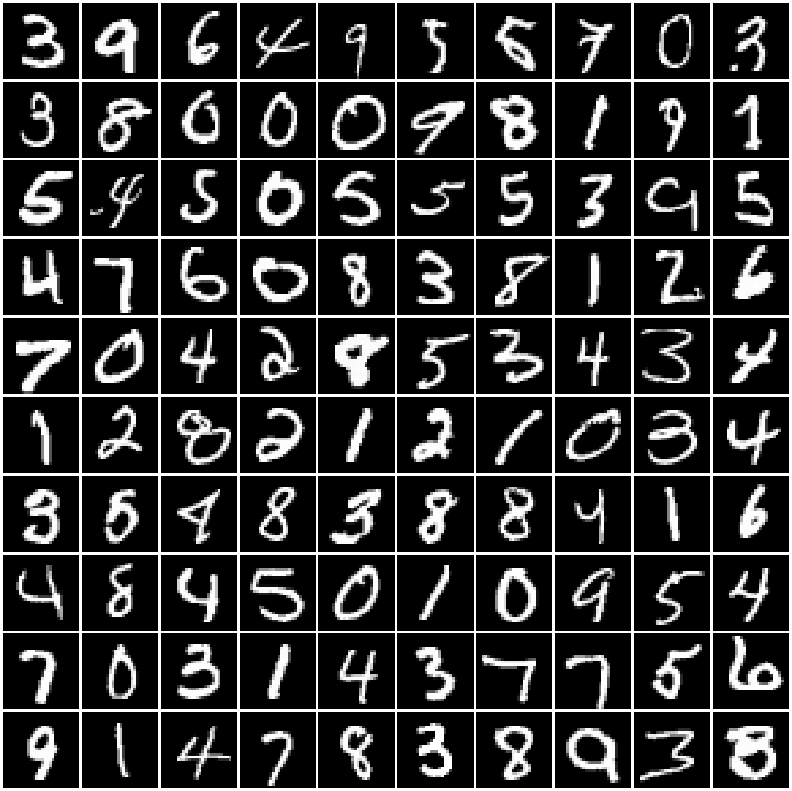
\includegraphics[width=0.40\textwidth]{thesis_data/mnist_example.png}
  \label{fig:MNISTExample}
}
\subfigure[A subsample from the SmallNORB dataset]{
  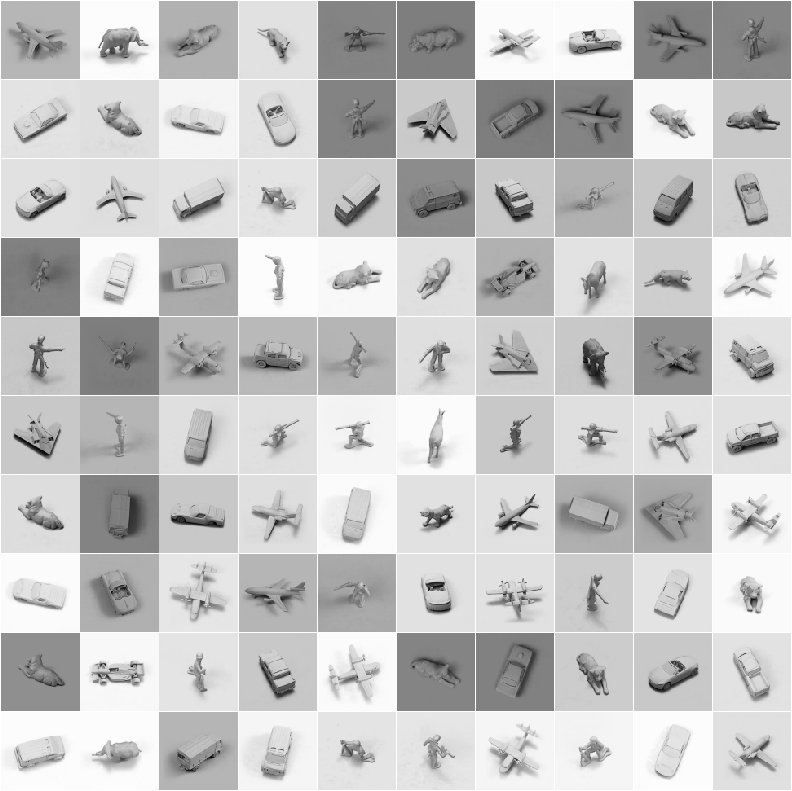
\includegraphics[width=0.40\textwidth]{thesis_data/norbsmall_example.png}
  \label{fig:NORBSmallExample}
}
\subfigure[MNIST patches]{
  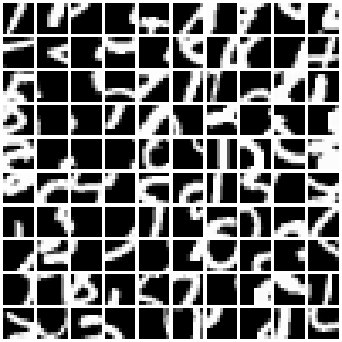
\includegraphics[width=0.40\textwidth]{thesis_data/mnist_patches.png}
  \label{fig:MNISTPatches}
}
\subfigure[SmallNORB patches]{
  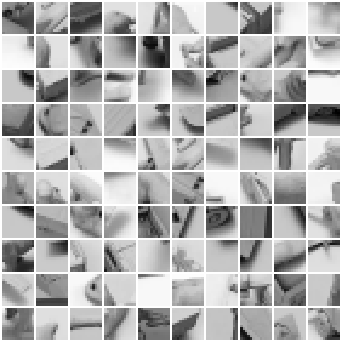
\includegraphics[width=0.40\textwidth]{thesis_data/norbsmall_patches.png}
  \label{fig:NORBSmallPatches}
}
\subfigure[MNIST patches with ZCA applied]{
  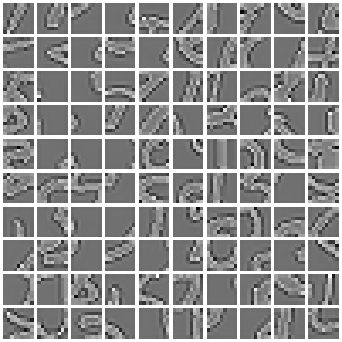
\includegraphics[width=0.40\textwidth]{thesis_data/mnist_patches_zca.png}
  \label{fig:MNISTPatchesZCA}
}
\subfigure[SmallNORB patches widt ZCA applied]{
  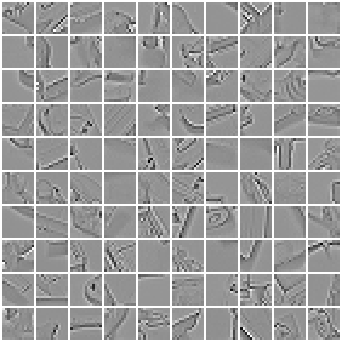
\includegraphics[width=0.40\textwidth]{thesis_data/norbsmall_patches_zca.png}
  \label{fig:NORBSmallPatchesZCA}
}
\caption{Subsamples and patches from MNIST and SmallNORB. The \textbf{ZCA} transformed patches in row three correspond to the original patches in row two.}
\label{fig:ViewsOfMNISTAndNORBSmall}
\end{figure}

\clearpage

\section{Coding, Reconstruction and Sparseness}

In this section we will talk again about coding methods, and compare their reconstructive and sparseness inducing powers. A set of $1000$ patches from the SmallNORB dataset will be used for evaluating the different methods. We will work with five feature sets, which we assume are given: a set of $w=169$ random features, a set of $w=169$ \textbf{PCA} features, a set of $w=169$ sparse features, anoter set of $w=512$ random features and another set of $w=512$ sparse features. The first three sets are critically-complete while the last two are roughly three times overcomplete. No overcomplete \textbf{PCA} feature set could, of course, be built. The \textbf{PCA} and sparse $w=169$ sets can be seen in \textbf{Figure \ref{fig:RecSparseFeatureSets}}. The larger sparse feature set is similar to the one shown. The coding methods we are interested in are inner product (\textbf{Corr}), \textbf{MP}, \textbf{OMP}, \textbf{OOMP} and SparseNet with $S(x) = \log(1 + x^2)$.

\begin{figure}
\centering
\subfigure[PCA feature set with $w=169$.]{
  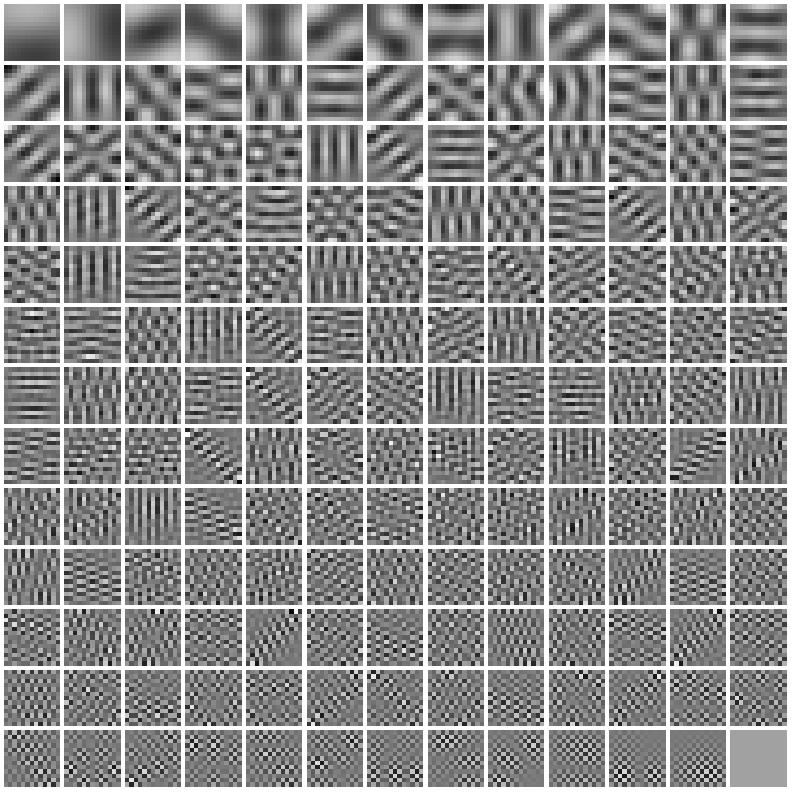
\includegraphics[width=0.45\textwidth]{thesis_data/recsparse/features_pca.png}
  \label{fig:RecSparseFeaturesPCA}
}
\subfigure[Sparse feature set with $w=169$.]{
  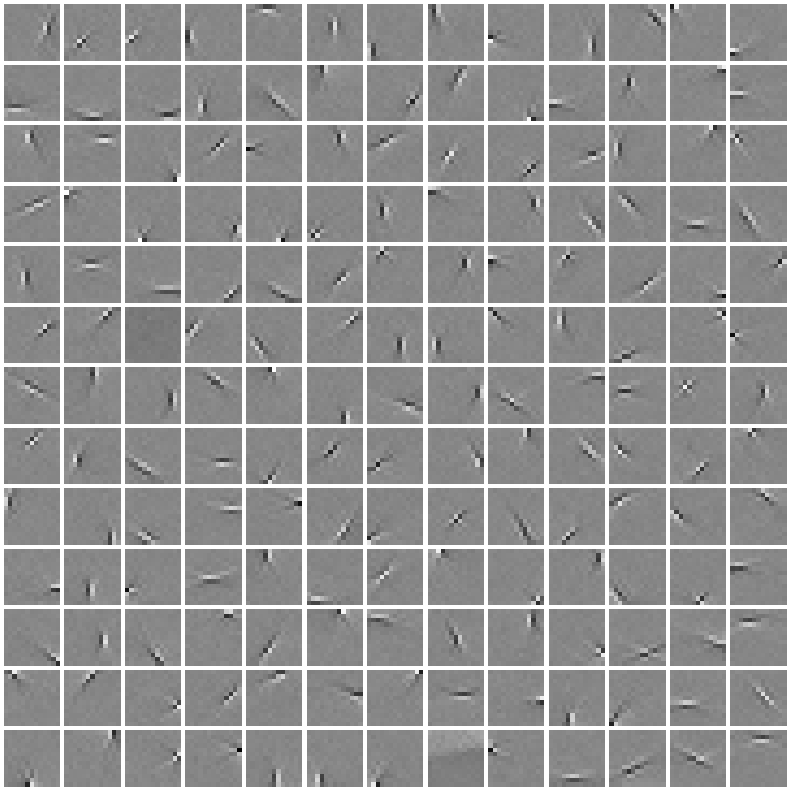
\includegraphics[width=0.45\textwidth]{thesis_data/recsparse/features_sparse.png}
  \label{fig:RecSparseFeaturesSparse}
}
\caption{Two of the three non-random feature sets employed in this section's experiments.}
\label{fig:RecSparseFeatureSets}
\end{figure}

In order to test the reconstruction power of the five coding methods we will measure the average squared sum of differences between an original patch $\textbf{x}$ and a reconstructed patch $\textbf{C}\textbf{a}$. That is, the average Euclidean norm of the error patch $\textbf{x} - \textbf{C}\textbf{a}$. We use the conventions estabilished in the chapter about coding methods. More precisely, $\textbf{C}$ is one of the five feature sets while $\textbf{a}$ is the code word obtained by applying one of the five coding methods we're testing to $\textbf{x}$ and $\textbf{C}$.

For this experiment we will constrain the reconstructive powers of the methods by imposing at most $k$ non-null coefficients. For \textbf{Corr} and SparseNet, the method will be allowed to run as usual, then the $k$ greatest coefficients in absolute value will be selected. \textbf{MP}, \textbf{OMP} and \textbf{OOMP} have $k$ builtin, therefore they suffer no modification. We will have five different values for $k$, namely, $1$, $3$, $16$, $64$ and $w$. When $k=1$ we will have a very strict coding setup. Basically, for a given $\textbf{x}$, $\textbf{a}$ will be zero everywhere except at the index $\omega$ corresponding to the most similar feature from $\textbf{C}$ to $\textbf{x}$. The similarity will be measured by inner-product / projection size of $\textbf{x}$ onto $\textbf{C}^\omega$. We expect \textbf{Corr}, \textbf{MP}, \textbf{OMP} and \textbf{OOMP} to produce the same results, as, for $k=1$, algorithmically speaking, there are no differences between the methods - even the least squares problems \textbf{OMP} and \textbf{OOMP} solve are reduced to inner product comparisons in such a limit case. When $k=3$ we will again have a very strict coding setup, though not as harsh as for $k=1$. We expect large errors in these two situations. For $k=16$ and $k=64$, differences between the methods will start to become apparent and we expect small errors. For $k=w$ we should see in a lot of methods and under a lot of feature sets the error reduced to $0$. For \textbf{OMP} and \textbf{OOMP}, in this case we'll have $k=169$, because, by their very construction, these methods guarantee a $0$ norm residual after $k=d$ steps, therefore every coefficient of $a$ for $t \ge d$ will necessarily be $0$. There is no point in wasting computational resources computing them.

\renewcommand{\arraystretch}{1.2}
\begin{table}
  \caption{Average reconstruction error for different coding methods and different feature sets.}
  \label{table:RecSparseErrors}
  \newcolumntype{R}{>{\centering}X}
  \begin{tabularx}{\textwidth}{|R|R|c|c|c|c|c|}
    \hline
    Features & Method & $k=1$ & $k=3$ & $k=16$ & $k=64$ & $k=w$ \tabularnewline \hline\hline
    \multirow{5}{*}{Random $w=169$} & \textbf{Corr} & $1.95$  & $1.88$ & $1.72$ & $1.81$ & $1.93$ \tabularnewline
    & \textbf{MP} & $1.95$ & $1.87$ & $1.57$ & $1.14$ & $0.87$ \tabularnewline
    & \textbf{OMP} & $1.95$ & $1.87$ & $1.55$ & $0.93$ & $0.00$ \tabularnewline
    & \textbf{OOMP} & $1.95$ & $1.87$ & $1.55$ & $0.93$ & $0.00$ \tabularnewline
    & SparseNet & $1.97$ & $1.93$ & $1.79$ & $1.58$ & $1.50$ \tabularnewline \hline
    \multirow{5}{*}{\textbf{PCA} $w=169$} & \textbf{Corr} & $1.47$ & $1.07$ & $0.55$ & $0.20$ & $0.00$ \tabularnewline
    & \textbf{MP} & $1.47$ & $1.07$ & $0.55$ & $0.20$ & $0.00$ \tabularnewline
    & \textbf{OMP} & $1.47$ & $1.07$ & $0.55$ & $0.20$ & $0.00$ \tabularnewline
    & \textbf{OOMP} & $1.47$ & $1.07$ & $0.55$ & $0.20$ & $0.00$ \tabularnewline
    & SparseNet & $1.58$ & $1.30$ & $1.01$ & $0.91$ & $0.90$ \tabularnewline \hline
    \multirow{5}{*}{Sparse $w=169$} & \textbf{Corr} & $1.76$ & $1.62$ & $1.25$ & $1.03$ & $1.04$ \tabularnewline
    & \textbf{MP} & $1.76$ & $1.61$ & $1.17$ & $0.57$ & $0.16$ \tabularnewline
    & \textbf{OMP} & $1.76$ & $1.61$ & $1.16$ & $0.50$ & $0.00$ \tabularnewline
    & \textbf{OOMP} & $1.76$ & $1.61$ & $1.16$ & $0.50$ & $0.00$ \tabularnewline
    & SparseNet & $1.83$ & $1.74$ & $1.51$ & $1.29$ & $1.24$ \tabularnewline \hline
    \multirow{5}{*}{Random $w=512$} & \textbf{Corr} & $1.93$ & $1.84$ & $1.71$ & $2.59$ & $5.20$ \tabularnewline
    & \textbf{MP} & $1.93$ & $1.83$ & $1.40$ & $0.68$ & $0.01$ \tabularnewline
    & \textbf{OMP} & $1.93$ & $1.83$ & $1.37$ & $0.44$ & $0.00$ \tabularnewline
    & \textbf{OOMP} & $1.93$ & $1.83$ & $1.37$ & $0.43$ & $0.00$ \tabularnewline
    & SparseNet & $1.96$ & $1.93$ & $1.78$ & $1.47$ & $0.89$ \tabularnewline \hline
    \multirow{5}{*}{Sparse $w=512$} & \textbf{Corr} & $1.75$ & $1.62$ & $1.98$ & $3.84$ & $7.02$ \tabularnewline
    & \textbf{MP} & $1.76$ & $1.53$ & $0.99$ & $0.40$ & $0.00$ \tabularnewline
    & \textbf{OMP} & $1.76$ & $1.53$ & $0.95$ & $0.26$ & $0.00$ \tabularnewline
    & \textbf{OOMP} & $1.76$ & $1.53$ & $0.95$ & $0.25$ & $0.00$ \tabularnewline
    & SparseNet & $1.88$ & $1.78$ & $1.56$ & $1.23$ & $0.80$ \tabularnewline \hline
  \end{tabularx}
\end{table}
\renewcommand{\arraystretch}{1.0}

\clearpage

A summary  of the results can be seen in \textbf{Table \ref{table:RecSparseErrors}}. Only the means are presented, however. The variances tended to be the same across methods and feature sets, and were roughly $0.40$ for $k=1$, $k=3$ and $k=16$, $0.10$ for $k=64$ and $0$ for $k=w$, except for SparseNet, which had a $0.10$ variance for this case as well. Several observations need to be made. First, regardless of feature set, reconstruction error goes down from \textbf{Corr} to \textbf{MP} to \textbf{OMP} to \textbf{OOMP}. Furthermore, for \textbf{Corr}, the error increases when  using random features. This breakdown is explained by the nature of the feature set - there is no simple structure to exploit - and the nature of the method - it cannot find ``hidden'' structure. When employing the sparse feature set with $w=169$, which does have some structure to it, the error drops to about half for $k=w$. For the overcomplete sparse set, however, the error radically increases. This is a sign of the severe limitations of the method - even with some structure it cannot produce a suitable approximation when there are more features than dimensions in the signal space. The \textbf{PCA} feature set presents itself in a form which \textbf{Corr} can handle. Therefore, for $k=w$ we have a zero error. More importantly, all methods which are somehow based on inner-products have the same behaviour for this feature set. With regards to inner-product based methods, \textbf{MP} handles itself well. For smaller $k$s it is roughly equivalent to the more complex methods. Better results are obtained in the overcomplete feature sets (both random and sparse) than the critically-complete one. For the overcomplete ones, at $k=512$ a zero error is actually reached. This means the bigger feature set allowed the method a way to find the certain features which allow a perfect reconstruction. The other two methods, \textbf{OMP} and \textbf{OOMP} behave roughly the same. \textbf{OOMP} seems to be a little bit better (by $0.01$ in some cases), but such a small difference would not recommend the method, from a purely approximation power point of view, given its increased compuational demands. As expected, when $k=169$ (the maximum useful for these methods, regardless of the actual $w$), the reconstruction is perfect, regardless of the feature set used. SparseNet does not produce very good approximations. Visual inspection of the result usually hints that there is a scale problem, rather than a shape problem. Also, the overcomplete sparse feature sete is the one which induces best results for this method, although the \textbf{PCA} set is not that far off.

\textbf{Figure \ref{fig:RecSparsePictures}} gives an ideea of the quality of a reconstructed patch, relative to the original. Notice that the patches corresponding to the random bases are more noisy than the other ones and that the patches corresponding to \textbf{PCA} are very similar to the original, regardeless of coding method. Also, the features of the SparseNet patches are barely percievable, even though a closer inspection will reveal the same general shape. This is caused by the previously mentioned amplitude problems.

\begin{figure}
\centering
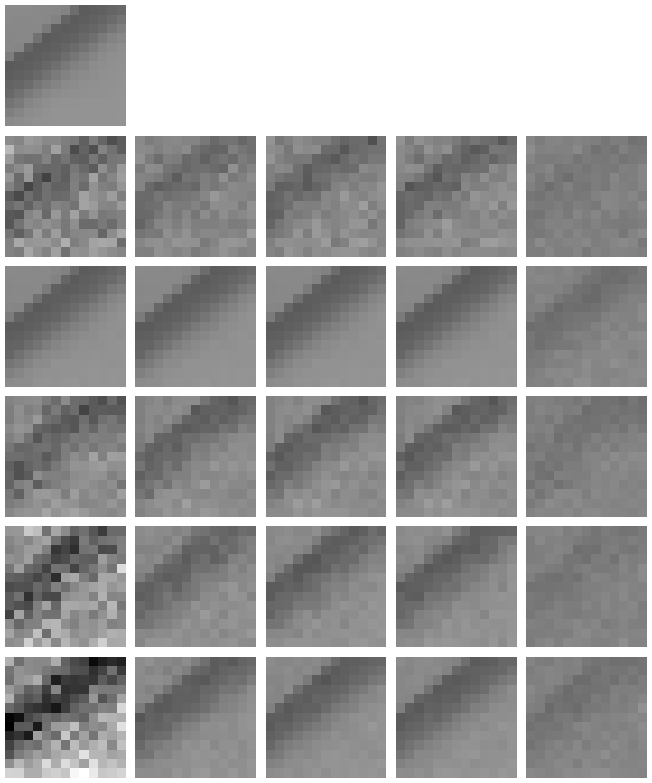
\includegraphics[width=0.95\textwidth,height=0.8\textheight]{thesis_data/recsparse/rec_pictures.png}
\caption{Reconstructions of the patch in the top-left corner using different coding methods and feature sets, but with fixed $k=64$. Each column handles one coding method. They are in order: \textbf{Corr}, \textbf{MP}, \textbf{OMP}, \textbf{OOMP} and SparseNet. Each row, after the first one,  handles one feature set. They are in order: random features with $w=169$, \textbf{PCA} features with $w=169$, sparse features with $w=169$, random features with $w=512$ and sparse features with $w=512$.}
\label{fig:RecSparsePictures}
\end{figure}

Reconstruction power is just one measure of the quality of a coding method, however. Another, arguably more important (cite here), measure is sparseness. One way to define spareness is to count how many zeros the code word $a$ has and express it relative to $w$. In practice, we care that a coefficient is ``large enough'', say, grater in absolute value than a small positive real $\delta$, rather than simply different from $0$. In our experiments, we set $\delta$ to $0.01$. More formally, we have:

\begin{equation*}
\rho(a) = \frac{\left| \{ a_i \left|\right. i \in \hcrange{1}{w} \wedge \left|a_i\right| > \delta \} \right|}{w} \in [0,1]
\end{equation*}

As in the last experiment, where we were interested in the average reconstruction error, we are now interested in the average sparseness. We continue with the same experimental setup as before. However, we will not impose a small $k$, but rather use $k=w$ or $k=d$, depending on the particular method. Imposing a $k \ll w$ would have artificially restricted the spareness and we would have gotten useful results only for larger values of $k$, for which the methods would be able to induce their own spareness. 

\renewcommand{\arraystretch}{1.2}
\begin{table}
  \caption{Average sparseness for different coding methods and different feature sets.}
  \label{table:RecSparseSparseness}
  \newcolumntype{R}{>{\centering}X}
  \begin{tabularx}{\textwidth}{|R|c|c|c|c|c|}
    \hline
    Features & \textbf{Corr} & \textbf{MP} & \textbf{OMP} & \textbf{OOMP} & SparseNet \tabularnewline \hline\hline
    Random $w=169$ & $0.48$ & $0.50$ & $0.50$ & $0.50$ & $0.41$ \tabularnewline \hline
    \textbf{PCA} $w=169$ & $0.36$ & $0.36$ & $0.36$ & $0.36$ & $0.38$ \tabularnewline \hline
    Sparse $w=169$ & $0.46$ & $0.50$ & $0.45$ & $0.45$ & $0.42$ \tabularnewline \hline
    Random $w=512$ & $0.47$ & $0.28$ & $0.13$ & $0.13$ & $0.37$ \tabularnewline \hline
    Sparse $w=512$ & $0.47$ & $0.19$ & $0.12$ & $0.12$ & $0.35$ \tabularnewline
    \hline
  \end{tabularx}
\end{table}
\renewcommand{\arraystretch}{1.0}

A summary of the results can be seen in \textbf{Table \ref{table:RecSparseSparseness}}. For the critically-complete random feature set every inner-product bases method performs roughly the same. SparseNet is significantly better, though, in general, all methods perform rather poorly, requiring about half of the coefficients to be greater than $\delta$. With \textbf{PCA} features, we again see the identical behaviour for all inner-product based methods. All methods have roughly the same behaviour, which is visibly better than with the random features, but not that great in general. Similarly, with the critically-complete sparse feature set, about half of the code word coefficients are active, regardless of method. However, \textbf{MP} is a little bit worse than \textbf{Corr} and the other pursuits. It probably can't find good matches in this limited feature set. SparseNet again leads the pack with performance similar to the random feature set case. When we move to the larger feature sets, however, the situation changes drastically. \textbf{Corr} remains at roughly the same level as with the $w=169$ feature sets, and SparseNet is slighly better, but the pursuits come into their own and produce very sparse results. Again, \textbf{OMP} and \textbf{OOMP} produce ``identical'' results, furthering our belief that the second has no practical advantage over the first. \textbf{MP} is roughly half as good as \textbf{OMP} and \textbf{OOMP}, especially in the random feature set, but is much better than simple correlation. Notice that, in absolute terms, in the best cases, roughly $60$ coefficients are needed for a good reconstruction, as $\hctimes{0.50}{128} \approx \hctimes{0.12}{512} \approx 60$. This is useful information for later experiments. Using a $k > 60$ with a $d$ similar to the ones we used in these experiments, will, most likely, not produce better results.

\begin{figure}
\centering
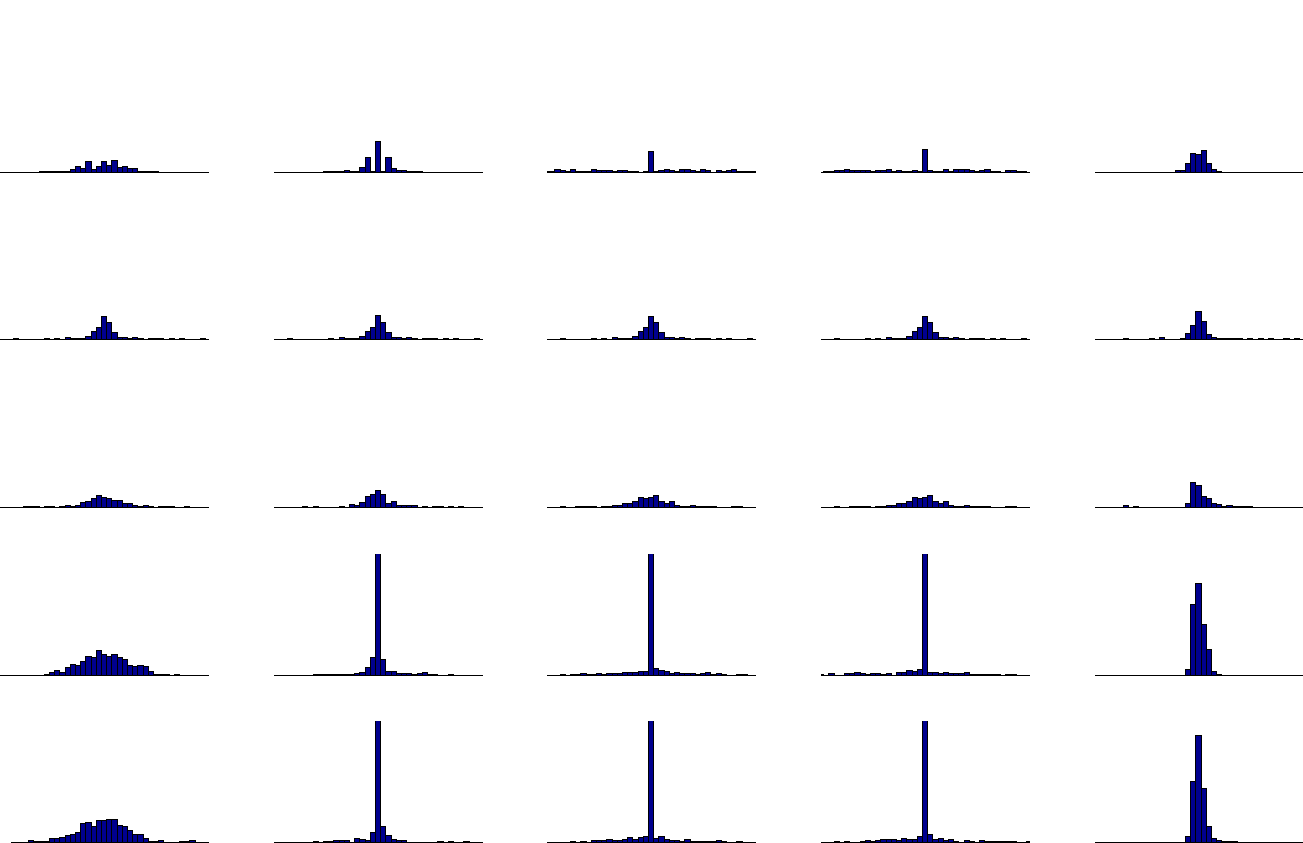
\includegraphics[width=0.95\textwidth,height=0.8\textheight]{thesis_data/recsparse/rec_hists.png}
\caption{Histograms of the code words for the patch in the top-left corner of \textbf{Figure \ref{fig:RecSparsePictures}} produced using different coding methods and feature sets. Each column handles one coding method. They are in order: \textbf{Corr}, \textbf{MP}, \textbf{OMP}, \textbf{OOMP} and SparseNet. Each row handles one feature set. They are in order: random features with $w=169$, \textbf{PCA} features with $w=169$, sparse features with $w=169$, random features with $w=512$ and sparse features with $w=512$. All horizontal axes are between $[-1.5,1.5]$ and all vertical ones are between $[0,250]$.}
\label{fig:RecSparseHists}
\end{figure}

\textbf{Figure \ref{fig:RecSparseHists}} gives an ideea of the distribution of the patches in the different cases. We used $61$ bins spread evenly in the interval $[-1.5,1.5]$. Notice how spiked the distributions for the pursuits are, expecially for \textbf{OMP} and \textbf{OOMP}. Again, these two produce almost identical results. The distribution for \textbf{Corr} is however very flat. \textbf{MP} is situated somewhat between these two extremes, but with a clear peak around $0$. Similarly, SparseNet has a peak around $0$, but the distribution has a skwed form, resulting from the regularization term we used. The effect is good, although the sparsity is clearly more strinking in the \textbf{OMP} and \textbf{OOMP} methods. The \textbf{PCA} features do not produce very ``sparse'' looking histograms, regardless of the methods employed, despite good reconstruction performance and acceptable average sparseness. Real sparseness is to be found in the way the values are distributed - there must be just a few code word coefficients with large values, besides being a lot of them equal to or near $0$.

\section{Learning Feature Sets}

Here we should talk about how we learn the feature sets for the different algorithms, and how they differ. Several feature sets should be showed as well as the parmeters used for learning them. Talk about how the interaction with each coding method works.

As we've seen, the difference between coding with dictionaries produced by different methods is not that great, if the dictionaries are of sufficient quality, and stems mostly from variations in the dictionaries produced and not in some intrinsic properties of the feature sets produced by one method versus the ones produced by another method. Where it is useful to compare methods is first in the ability to learn very over-complete feature sets for large $d$s and with not that many patches and execution speed.

\section{Coder Architecture Evaluation}

The MNIST database (cite source here) is used for handwritten digit recognition. It consists of $\hctimes{28}{28}$ grayscale images of the digits from $0$ to $9$. Examples for each class can be seen in Figure (figure). There are $60000$ training images and $10000$ test images. It is frequently used as a benchmark for classifier systems, although, as the score reference in (cite site with scores) will attest, the practical limits have been reached. Nevertheless, the system we built, especially using the Global Order nonlinearity, were able to break the record on this database, for the case of a non-modified dataset.

We did several experiments. The goal was to get a classification score as high as possible. A summary of the best methods so far, as gathered from mnist site and ciresan site can be seen in table.

First, to get a good reference we employed a one-vs-one trained linear svm in primal mode with L2 loss and L2 regularization as implemented by LIBSVM and trained it on the raw data. We also did a version with standardized and normalized data, with slightly better results. The results can be seen in table (table here). There is just one tunable parameter, $C$ and its value is determined by crossvalidation. The experiment was carried out as such: first, $C$ was determined by cross-validation. To this end, $20$\% of the training dataset was selected. Then, $5$ splits into training and validation datasets were made, keeping $75$\% of this for training and the other $25$\% for validation. Thus, we did five-fold cross-validation. These splits were kept constant and each value of $C$, which was logarithmically spread between $10^{-2}$ and $1$ with $20$ points to test, was trained on the $5$ training subsamples and evaluated on the $5$ validation subsamples. Once this was done, the average of the validation scores was used to select the best $C$ (the one with the highest score). The graph in figure ... shows the score plot for different $C$ and the associated standard deviations. After a best $C$ was found, another SVM was trained on the full training set (and with the associated $C$) and the final score was produced on the test set. The table presents both final scores and crossvalidation average score for best $C$ as well as best $C$. This general model of classification will be used for all other experiments, except where otherwise noted.

Another experiment we ran showed the power of the Global Order nonlinearity. More precisely, after a few experiments, we determined a configuration for the coder which produced state of the art results for the MNIST dataset, in the case of not employing any modifications to the dataset (elastic distorsions etc. which would increase the size of the machine) and u sing just one classifier. The general architecture uses $2048$ randomly built bases and coding with correlation limited to $k=100$ coefficients. The patch size is $p=9$. The nonlinearity was global order, with the smallest value set to $0.01$. No polarity splitting was done. The reduce method was $SumSqr$ and the reduce spread was $4$. The score we got was $99.53$, which is greater than the biggest got so far. If we use more than one classifiers, for example if we use $7$ of them in parallel, and take the class with the most votes (the mode of the distribution), then we can push the results up to .... This is because of using random bases. Just like with boosting or Random Trees (cite random trees article here), introducing randomness and then taking the results of many many random units produces better results. The results are summarised in table ...

Decide if to talk about bigger datasets here or not.

To get a feel for which setups are good and which are bad, more exhaustive experiments are needed. This is what we'll do in this next section.

Testing every combination of architecture we can imagine for the systems is prohibitive at best. Therefore an full factorial experiment is out of the question. We split the experiments into three parts, which, by intuition and experience seem to be roughly independent. First the overal coding strategy used. We will test {random bases|dct bases|gabor bases|grad bases|neural gas} x {corr|mp|omp|oomp} x {linear|logistic|global order}. All other parameters will be kept constant at seemengly OK levels. After the best coding setup for this experiment is done, we will investigate how the number of features as well as the controllable sparseness ($k/w$) affects performance. Either the best or several of the best methods in the last experiment will be used (especially if the differences are small). Finally, the properties of the coding geometry and reduce type and reduce geometry will be studied. Also, questions about polarity splitting will be used as well and how they behave.

We are not always interested in best absolute performance. Consider the text detection application we'll talk about later. If we want real-time performance, we have to impose tight constraingts on the compuational budget. We want an architecture which performs well under these constraints. We therefore face a multi-objective optimization problem, of sorts. We prefere, for example, for computational reasons, smaller patch sizes. If we employ a size of, say, $p=3$ or $p=5$, then a correlation with such a filter can be hard-coded instead of written as a loop and could also fit in the vectorization units of moder processors. However, such a small patch size is unlikely to capture much information from an image, so, in general, and as the tables, show, just using small patches will yield poor performance. However, if certain other architectural decisions, like using the Global Order nonlinearity or using a MaxKeepSign and KeepSign polarities, help us reach good or almost-good performance, we should use them. Not all applications have these constraints however, so for a medical diagnosis problem, accuracy would be primary.

\chapter{Text Detection Application}

\chapter{Conclusions}

\bibliographystyle{unsrt}
\bibliography{Bibliography}

\appendix

\end{document}
